%%%%%%%%%%%%%%%%%%%%%%%%%%%%%%%%%%%%%%%%%%%%%%%%%%%%%%%%%%%%%%%%%%
%%%%%%%% ICML 2012 EXAMPLE LATEX SUBMISSION FILE %%%%%%%%%%%%%%%%%
%%%%%%%%%%%%%%%%%%%%%%%%%%%%%%%%%%%%%%%%%%%%%%%%%%%%%%%%%%%%%%%%%%

% Use the following line _only_ if you're still using LaTeX 2.09.
%\documentstyle[icml2012,epsf,natbib]{article}
% If you rely on Latex2e packages, like most moden people use this:
\documentclass{article}

% For figures
\usepackage{graphicx} % more modern
%\usepackage{epsfig} % less modern
\usepackage{subfigure}
\usepackage{mathtools}
\usepackage{amssymb}
\usepackage{natbib}
\usepackage{algorithm}
\usepackage{algorithmic}
\usepackage{amsthm}
\usepackage{hyperref}
\usepackage{url}
\newcommand{\theHalgorithm}{\arabic{algorithm}}
\usepackage{icml2012}
\mathtoolsset{showonlyrefs=true}

\newtheorem{definition}{Définition}
\newtheorem{lemme}{Lemma}
\newtheorem{theorem}{Théorème}
\newtheorem{hypo}{Hypothèse}
\newtheorem{cor}{Corollaire}
\newtheorem{prop}{Proposition}
\newtheorem{exemple}{Exemple}
\newtheorem{remarques}{Remarques}
\newtheorem{remarque}{Remarque}
\newtheorem{assumption}{Assumption}
\newtheorem{problem}{Problème}
\newtheorem{algo}{Algorithme}
\newtheorem{preuve}{Démonstration}
\newcommand{\argmax}{\operatorname*{argmax}} %\operatorname* pour les op. pouvant admettre des limites...
\newcommand{\argmin}{\operatorname*{argmin}}
\newcommand{\minp}{\operatorname*{min_+}}
\newcommand{\dom}{\operatorname*{dom}}
\newcommand{\Ker}{\operatorname*{Ker}}
\newcommand{\trace}{\operatorname*{trace}}
\newcommand{\cov}{\operatorname{cov}}
\newcommand{\epi}{\operatorname{epi}}
\newcommand{\card}{\operatorname*{Card}}
\newcommand{\conv}{\operatorname*{Conv}}
\newcommand{\vect}{\operatorname*{Vect}}
\newcommand{\var}{\operatorname{Var}}
\newcommand{\diag}{\operatorname{diag}}
\newcommand{\erf}{\operatorname{erf}}
\newcommand{\bound}{\operatorname*{bound}}
\newcommand{\vpi}{\operatorname{VPI}}
\newcommand{\gn}{\operatorname{Gain}}
\newcommand{\p}{\operatorname{Pr}}
\newcommand{\mlp}{\operatorname{MLP}}
\newcommand*\tto[2]{\smash{\mathop{\longrightarrow}\limits_{#1}^{#2}}}
\newcommand*\ntto[2]{\smash{\mathop{\nrightarrow}\limits_{#1}^{#2}}}
\newcommand{\X}{\mathbf{X}}
\newcommand{\Q}{\mathbf{Q}}
\newcommand{\A}{\mathbf{A}}
\newcommand{\Z}{\mathbf{Z}}
\newcommand{\Y}{\mathbf{Y}}
\newcommand{\E}{\mathbf{E}}
\newcommand{\K}{\mathbf{K}}
\newcommand{\F}{\mathcal{F}}
\newcommand{\R}{\mathbf{R}}
\newcommand{\ba}{\mathbf{a}}
\newcommand{\bb}{\mathbf{b}}
\newcommand{\bc}{\mathbf{c}}
\newcommand{\bd}{\mathbf{d}}
\newcommand{\be}{\mathbf{e}}
\newcommand{\af}{\mathbf{f}}
\newcommand{\bg}{\mathbf{g}}
\newcommand{\bh}{\mathbf{h}}
\newcommand{\bi}{\mathbf{i}}
\newcommand{\bj}{\mathbf{j}}
\newcommand{\bk}{\mathbf{k}}
\newcommand{\bl}{\mathbf{l}}
\newcommand{\bm}{\mathbf{m}}
\newcommand{\bn}{\mathbf{n}}
\newcommand{\bo}{\mathbf{o}}
\newcommand{\bp}{\mathbf{p}}
\newcommand{\bq}{\mathbf{q}}
\newcommand{\br}{\mathbf{r}}
\newcommand{\bs}{\mathbf{s}}
\newcommand{\bt}{\mathbf{t}}
\newcommand{\bu}{\mathbf{u}}
\newcommand{\bv}{\mathbf{v}}
\newcommand{\bw}{\mathbf{w}}
\newcommand{\bx}{\mathbf{x}}
\newcommand{\by}{\mathbf{y}}
\newcommand{\bz}{\mathbf{z}}
\newcommand{\ma}{\mathbf{A}}
\newcommand{\mb}{\mathbf{B}}
\newcommand{\mc}{\mathbf{C}}
\newcommand{\md}{\mathbf{D}}
\newcommand{\me}{\mathbf{E}}
\newcommand{\mf}{\mathbf{F}}
\newcommand{\mg}{\mathbf{G}}
\newcommand{\mh}{\mathbf{H}}
\newcommand{\mi}{\mathbf{I}}
\newcommand{\mj}{\mathbf{J}}
\newcommand{\mk}{\mathbf{K}}
\newcommand{\ml}{\mathbf{L}}
\newcommand{\mm}{\mathbf{M}}
\newcommand{\mn}{\mathbf{N}}
\newcommand{\mo}{\mathbf{O}}
\newcommand{\Mp}{\mathbf{P}}
\newcommand{\mq}{\mathbf{Q}}
\newcommand{\mr}{\mathbf{R}}
\newcommand{\ms}{\mathbf{S}}
\newcommand{\mt}{\mathbf{T}}
\newcommand{\Mu}{\mathbf{U}}
\newcommand{\mv}{\mathbf{V}}
\newcommand{\mw}{\mathbf{W}}
\newcommand{\mx}{\mathbf{X}}
\newcommand{\my}{\mathbf{Y}}
\newcommand{\mz}{\mathbf{Z}}
\newcommand{\tphi}{\tilde{\Phi}}
\newcommand{\espace}{\text{ }}


\newcommand{\x}{\mathbf{x}}
\newcommand{\s}{\mathbf{s}}
\newcommand{\n}{\mathbf{n}}
\newcommand{\y}{\mathbf{y}}
\newcommand{\I}{\mathbf{I}}
\newcommand{\rr}{\mathbf{r}}

%%%%%%%%%%%%%%%%%%%%%%%%%%%%%%%%%%%%%%%%%%%%%%%%%%%%%%%%%%%%%%%%%%%%%%%
% Titre court si le titre fait plus de 40 caractères
%%%%%%%%%%%%%%%%%%%%%%%%%%%%%%%%%%%%%%%%%%%%%%%%%%%%%%%%%%%%%%%%%%%%%%%

%\shorttitle{Classification structurée pour l'ARI}
%
%\shortouvrage{CAp 2012}

% Titre, auteur, pas de date

%\title{Classification structurée pour l'apprentissage par renforcement inverse}
%
%\author{\fontsize{12}{12}\selectfont{Edouard Klein\inst{1}$^,$\inst{2}, Bilal Piot \inst{1}$^,$\inst{3}, Matthieu Geist\inst{1}, Olivier Pietquin\inst{1}$^,$\inst{3}}}
%
%\institute{
%Sup\'elec, IMS Research group, France, \texttt{prenom.nom@supelec.fr}
%\and
%Equipe ABC,
%LORIA, France
%\and
%UMI 2958
%GeorgiaTech-CNRS, France
%}
\icmltitlerunning{Structured Classification for Inverse
Reinforcement Learning}


\begin{document}

\twocolumn[ \icmltitle{Structured Classification for Inverse
Reinforcement Learning}

% It is OKAY to include author information, even for blind
% submissions: the style file will automatically remove it for you
% unless you've provided the [accepted] option to the icml2012
% package.
\icmlauthor{Your Name}{email@yourdomain.edu}
\icmladdress{Your Fantastic Institute,
            314159 Pi St., Palo Alto, CA 94306 USA}
\icmlauthor{Your CoAuthor's Name}{email@coauthordomain.edu}
\icmladdress{Their Fantastic Institute,
            27182 Exp St., Toronto, ON M6H 2T1 CANADA}

% You may provide any keywords that you
% find helpful for describing your paper; these are used to populate
% the "keywords" metadata in the PDF but will not be shown in the document
\icmlkeywords{inverse reinforcement learning, structured multi-class
classification}

\vskip 0.3in
]



\begin{abstract}
This paper addresses the Inverse Reinforcement Learning (IRL)
problem which is a particular case of learning from demonstrations.
The IRL framework assumes that an expert, demonstrating a task, is
acting optimally with respect to an unknown reward function to be
discovered. Unlike most of existing IRL algorithms, the proposed
approach doesn't require any of the following: complete trajectories
from the expert, a generative model of the environment, the
knowledge of the transition probabilities, the ability to repeatedly
solve the forward Reinforcement Learning (RL) problem, the expert's
policy anywhere in the state space. Using a classification approach
in which the structure of the underlying Markov Decision Process
(MDP) is implicitly injected, we end-up with an efficient
subgradient descent-based algorithm.
% whose computational and sample
%complexities are low.
In addition, only a small amount of expert
demonstrations (not even in the form of trajectories but simple
transitions) is required.
%A formal analysis of the algorithm as well as empirical
%demonstrations on two classic but challenging problems are provided.
\end{abstract}
%%%%%
\section{Introduction}
%%%%%
%Dans cette contribution, nous nous plaçons dans le contexte de l'apprentissage par démonstration. Dans ce cadre, un agent artificiel apprend à reproduire une tâche grâce à l'observation d'un expert réalisant cette tâche de manière optimale. Pour trouver une solution à ce problème, nous nous proposons d'utiliser le paradigme de l'apprentissage par renforcement inverse. On suppose alors que l'expert agit de manière à être récompensé pour son comportement relativement à une fonction de récompense inconnue. Le but de l'agent est alors d'inférer cette fonction des démonstrations données par l'expert pour ensuite optimiser son comportement relativement à cette fonction lui aussi.\\

This contribution addresses the problem of learning by watching or
learning from demonstrations. In this context, an artificial agent
learns to perform a task by observing an expert demonstrating the
task. In order to find a solution to this problem, the Inverse
Reinforcement Learning (IRL) paradigm has been
proposed~\cite{russell1998learning}. The fundamental idea of IRL is
that the expert acts so as to be rewarded by an unknown reward
function. The aim of the IRL agent is then to infer the unknown
reward function from the demonstrations given by the expert, the
reward being considered as the most compact representation of the
task to be transferred to the agent. This way, an optimal behavior
can be obtained in any situation by optimizing the action selection
process according to the reward function. Unlike supervised
learning, the agent may not purely imitate the expert's actions but
will try to accomplish the same task optimally.
%
%
%La littérature sur le sujet est assez récente et trouve sa genèse dans \cite{russell1998learning}. Plusieurs directions ont depuis été explorées à partir de deux articles fondateurs \cite{ng2000algorithms} et \cite{abbeel2004apprenticeship}.\\
%Dans cette littérature (voir \cite{neu2009training} pour un bon survol), plusieurs verrous sont identifiés mais souvent ignorés pour proposer des algorithmes de résolution. Particulièrement, on suppose souvent connue la dynamique de l'environnement dans lequel évoluent l'expert et l'agent ou bien la mise à disposition de cet environnement (ou d'un simulateur) pour y tester les effets d'une politique quelconque. De plus, ces approches supposent de résoudre le problème direct (optimiser une politique pour une récompense donnée) un grand nombre de fois pour résoudre le problème inverse (trouver une récompense expliquant la politique). De plus, certaines de ces approches donnent en sortie une politique généralisant celle de l'expert plutôt qu'une récompense l'expliquant. Ces contraintes sont souvent incompatibles avec la mise en oeuvre des algorithmes proposés sur des cas réels.\\
%
%
The literature on the subject is quite recent and finds its origin
in \cite{russell1998learning}. Different approaches have been
explored since the first articles on the matter
\cite{ng2000algorithms,abbeel2004apprenticeship}.

In this literature (see \cite{neu2009training} for a survey),
several bottlenecks are identified but often ignored when developing
algorithms. Specifically, the dynamic of the environment where the
expert and the agent are evolving is assumed to be known, or an
environment model (via a simulator) must be available so as to test
the effects of a policy. Moreover, most of existing approaches
require solving the direct reinforcement learning problem (find an
optimal policy knowing a given reward) several times. Finally, in
many cases, the output of the algorithm is a policy but not a unique
reward function which makes task transfer hard to realize. These
constraints can lead to the development of algorithms unapplicable
to real problems.
%Dans cette contribution, nous proposons une méthode de résolution du problème d'apprentissage par renforcement inverse s'affranchissant de toute connaissance additionnelle aux démonstrations fournies par l'expert. Nous proposons une preuve de convergence de cet algorithme et fournissons une expérimentation sur le problème du pendule inversé. Le choix de cette application se justifie par la difficulté  qu'elle pose pour les méthodes de résolution de la littérature.
%
In this paper, we propose a resolution method of the inverse
reinforcement problem that is free from any other knowledge than the
demonstrations given by the expert. The proposed approach, the
Structured Classification for IRL (SCIRL), relies on a
classification paradigm in which the structure of the environment's
dynamics is implicitly introduced. Sec.~\ref{back.sec}
and~\ref{biblio.sec} provide the necessary background and review a
part of the state of the art. Sec.~\ref{sec:scirl} introduces our
contribution and Sec.~\ref{proof.sec} analyses the asymptotic
algorithm. Section~\ref{exp.sec} shows results obtained on two
classical benchmarks: inverted pendulum and the highway driving
problems.
%
%A proof of the convergence of the algorithm is provided in
%Section~\ref{proof.sec} and Section~\ref{exp.sec} shows results
%obtained on two classical benchmarks: inverted pendulum and the
%highway driving problems. The choice of the first application is
%justified by the fact that it is hard to solve by the other methods.


%%%%
\section{Background}
%%%%%
\label{back.sec}
%%%
Let's start with some background on RL and IRL and settle the
notations.

\subsection{(Inverse) Reinforcement Learning}
%%%
%Le cadre dans lequel nous plaçons notre étude est celui de la prise de décisions séquentielles. La configuration du système à contrôler est alors complètement décrite à chaque instant discret $t$ par un état $s_t \in S$. Confronté à cet état, l'agent doit prendre un décision $a_t\in A$. Le système évolue alors vers l'état suivant $s_{t+1}$ selon une certaine probabilité de transition markovienne $p(s_{t+1}|s_t, a_t)$. Une politique de contrôle déterministe $\pi: S\rightarrow A$ définit le comportement d'un agent confronté à un tel problème de décisions séquentielles.\\

The problem is seen as a sequential decision making problem posed in
the Markov Decision Process (MDP) formalism. In this formalism, a
system to be controlled can reach different configurations
completely described at each discrete time $t$ by a state $s_t \in
S$. Given the knowledge of the state, the agent must take a decision
$a_t\in A$. Then, the system evolves to a next state $s_{t+1} \in S$
with the Markovian probability $p(s_{t+1}|s_t, a_t)$. %(in short
%$p(s'|s,a)$ where $s'=s_{t+1}, s=s_t$ and $a=a_t$).
A policy, which
is a function $\pi: S\rightarrow A$, defines the behavior of the
agent. In this paper all the policies considered are deterministic,
$S$ and $A$ will be finite sets and $\{P_{sa}\}_{s\in S,a\in A}$
will be a set of probability distributions, from $S$ to $[0,1]$ such
that $P_{sa}(s')=p(s'|s, a)$, called transition probabilities.
%
%Dans le cadre de l'apprentissage par renforcement,la résolution de ce problème est guidée par une fonction de récompense $R: S \rightarrow \mathbb{R}$ qui indique le degré de désirabilité de chaque état. Une des forces de ce cadre réside dans le fait que l'agent ne va pas apprendre à maximiser la récompense immédiate mais au contraire un critère prenant le futur en compte, ce qui permet de spécifier uniquement le but et non la façon de l'atteindre. On définit pour ce faire la fonction de valeur $V^\pi$:
%
The RL paradigm aims at solving the problem of finding the optimal
sequence of actions in an MDP. The optimality criterion is based on
the definition of a reward function $R: S \rightarrow \mathbb{R}$
which defines the immediate reward $R(s)$ given to the agent when
the system is in the state $s \in S$. The agent should not learn to
maximize the immediate reward but a criterion taking into account
future rewards. The criterion commonly chosen is the value function
$V^\pi$:
%
\begin{align}
\label{Vdef.eqn} V^\pi(s) & = E^\pi_s[\sum_{t\geq0}\gamma^tR(s_t)]\\
& = R(s) + \gamma\sum_{s'\in S}P_{s\pi(s)}(s') V^\pi(s'),
\end{align}
%où $\gamma \in [0,1)$ est un facteur d'actualisation. Il est également possible de définir une fonction de qualité qui ajoute un degré de liberté sur le choix de la première action:
%
where $\gamma \in [0,1)$ is a discount factor, and $E^\pi_s$ is the
expectation over the distribution of the state sequences
$(s_0,s_1,\dots)$ the agent passes through when executing the policy
$\pi$ starting from $s_0=s$. One can define the action-value
function $Q^\pi$ which adds a degree of freedom in the choice of the
first action:
%
\begin{align}
\label{Qdef.eqn} Q^\pi(s,a) & =
E^\pi_{sa}[\sum_{t\geq0}\gamma^tR(s_t)]\\
& = R(s) + \gamma\sum_{s'\in S}P_{sa}(s') V^\pi(s').
\end{align}
%
%where $E^\pi_{sa}$ is the expectation over the distribution of the
%state sequences $(s_0,s_1,\dots)$ we pass through when we start from
%$s_0=s$, choose the action $a_0=a$ and then follow the policy $\pi$.
%
%Une politique optimale $\pi^*$ est définie comme une politique dont la fonction de valeur (optimale) $V^*$ vérifie $\forall \pi, \forall s, V^*(s) \geq V^\pi(s)$. La politique optimale se calcule simplement à partir de la fonction de qualité optimale $Q^*$ via un mécanisme glouton:
%
An optimal policy $\pi^*$ is defined as a policy with maximal value
function, $V^{\pi*}=V^*=\sup_{\pi}V^{\pi}$, which means that
$\forall \pi, \forall s, V^{\pi*}(s) \geq V^\pi(s)$. An optimal
policy $\pi^*$ can be computed easily thanks to the optimal
action-value function $Q^{\pi*}=Q^*=\sup_{\pi}Q^\pi$ via a greedy
mechanism:
%
\begin{equation}
\label{greedy.eqn} \pi^*(s) \in \arg\max_{a\in A} Q^*(s,a).
\end{equation}
%L'ensemble formé par l'espace d'état $S$, l'espace d'action $A$, les probabilités de transition $p$, le facteur $\gamma$ et la fonction de récompense $R$ forme un processus décisionnel de Markov .\\
%
The tuple $M=\{S,A,\{P_{sa}\}_{s\in S,a\in A},\gamma,R\}$ is called
a finite MDP. Resolving the RL problem with respect to the criterion
$V^\pi$  means to find $\pi^*$, usually without the full knowledge
of the MDP but only by observing transitions and rewards. In a
finite MDP the existence of an optimal deterministic policy is
guaranteed when the reward function $R$ is bounded.
%
%Parfois, définir la fonction de récompense est une tâche ardue alors qu'il est possible à l'opérateur de convenablement contrôler le système de manière intuitive. Un exemple de ce type de tâche est la conduite d'une voiture. Nous accomplissons ce genre de chose au quotidien sans trop y penser mais nous serions bien en peine de préciser les poids précis que nous attribuons aux différents critères tels que la distance nous séparant de la voiture devant nous, la brutalité avec laquelle nous appuyons sur la pédale de frein lorsqu'un danger se présente et ainsi de suite. Dans de tels cas, il est utile d'inférer la récompense à partir d'un comportement démontré.\\
%
The optimal behaviour being defined relatively to the reward, it's
observation is mandatory to learn. Sometimes, specifying manually
the reward function can be a hard job while it is natural to an
operator to achieve the desired task. For instance, driving a car is
such a task. One can accomplish this task very easily in his
daily-life but it is very tricky to specify the precise weights
given to each important driving-parameters such as the distance to
keep with the leading car, the speed below which it is unreasonable
to drive and so on. In such cases, inferring the reward function
from observed behavior would be helpful.
%
%C'est la définition de l'apprentissage par renforcement inverse. Le problème est de retrouver la fonction de récompense optimisée par un expert. Usuellement l'expert est considéré comme un agent optimal dans un PDM et l'on a accès ou bien à la politique complète $\pi_E$ de l'expert ou bien à quelques trajectoires tirées selon cette politique.\\
%
It is the aim of IRL. The expert, demonstrating the task, is thus
considered as an optimal agent in a MDP and the IRL agent has access
to the expert optimal policy $\pi_E$ or to some trajectories drawn
from this policy.
%
%Ce problème est mal posé dans la mesure où il n'y a pas unicité de la récompense pour laquelle un comportement est optimal (\cite{ng1999policy}). Particulièrement, tout comportement est optimal vis-à-vis de la récompense uniformément nulle. Il convient donc de contraindre l'espace des solutions.
The problem of finding a reward function from expert demonstrations
in the IRL framework is ill-posed. Indeed, there is not uniqueness
of the reward function for which the expert policy is
optimal~\cite{ng1999policyreward}. Particularly, each policy is
optimal with respect to the uniformly-zero reward function. Some
solutions have to be favored.
%%%
\subsection{Feature expectation}
\label{ConsiderationsTechniques.sec}
%%%
%La récompense $R$ est l'inconnue du problème. Nous supposons que l'utilisateur est en mesure de fournir $p$ fonctions de base $\psi_{1\leq i \leq N}$  telles que
The actual expert reward function $R_E$ is unknown. The problem is
 thus to find a reward function $R_\theta$ for which the policy of
the expert is also optimal. Let's assume that, given a set of $p$
features $\psi: S\rightarrow \mathbb{R}^p$, each components of
$\psi$: $\{\psi_i\}_{1\leq i \leq p}$ being a basis function from
$S$ to $\mathbb{R}$, such a reward can be written:
\begin{equation}
\label{hatRdef.eqn} %\exists \theta |
R_\theta(s) = \theta^T\psi(s) =
\sum_{i=1}^p\theta_i\psi_i(s).
\end{equation}
%Cette contrainte peut cependant être relâchée si nécessaire. Introduire cette expression dans la définition de la fonction de qualité (Eq. \eqref{Qdef.eqn}) fait apparaître un terme intéressant et dont l'usage est assez répandu dans les algorithmes existants:
Using this expression allows rewriting (Eq. \eqref{Qdef.eqn}) as:
\begin{equation}
Q^\pi(s,a)=\theta^T\mu^\pi(s,a),\text{ }\mu^\pi(s,a) =
E^\pi_{sa}[\sum_{t\geq 0}\gamma^t\psi(s_t)]. \label{Qmu.eqn}
\end{equation}
%Le terme $\mu^\pi$ est appelé l'attribut vectoriel moyen ({\it feature expectation}) d'une politique. On peut voir que la paramétrisation choisie pour $R$ et la dynamique imposée par l'application de la politique $\pi$ dans le PDM fixe la paramétrisation de $Q^\pi$.\\
%
The term $\mu^\pi$ is called the feature expectation of the policy
$\pi$. We can observe that the chosen parametrization of the reward
function $R_\theta$ and the dynamics resulting from the application
of the policy $\pi$ in the MDP gives rise to an induced
parametrization for $Q^\pi$. To
shorten notations, we may use $\mu^\pi_{sa}$ as $\mu^\pi(s,a)$.\\
%
%On peut noter que si deux politiques ont le même attribut vectoriel moyen, alors ces deux politiques ont la même valeur vis-à-vis de la récompense, quel que soit le vecteur de poids $\theta$ définissant celle-ci. En effet
We see also note that if two policies share the same feature
expectation, then they have the same value function with respect to
any reward function $R_\theta=\theta^T\psi$,
$\theta\in\mathbb{R}^p$. Indeed:
%
\begin{equation}  \mu^{\pi_1} = \mu^{\pi_2} \Rightarrow
\theta^T\mu^{\pi_1} = \theta^T\mu^{\pi_2} \Rightarrow V^{\pi_1} =
V^{\pi_2}. \label{memevaleur.eqn}
\end{equation}
%
%L'attribut vectoriel moyen de l'expert, $\mu_E$, peut être calculé sans forcément avoir accès à l'intégralité de la politique $\pi_E$. La plupart des algorithmes de la littérature ont, comme nous allons le voir, pour objectif de minimiser la distance entre les attributs vectoriels moyens respectifs de l'agent et de l'expert. Cela permet d'obtenir un agent dont le comportement a la même fonction de valeur que celui de l'expert, quelle que soit la récompense (voir par exemple \cite{neu2009training}).
%
That is why most of the algorithms in the literature have, as we
will see, the objective of minimizing a \textit{distance}  between
the feature expectation of the expert and the feature expectation of
the apprentice. %That allows to obtain an apprentice which policy has
%the same value function as the expert policy, for a reward function
%of the type $R=\theta^T\psi,\forall \theta\in\mathbb{R}^p$ (see for
%instance
%~\cite{neu2009training}.

\section{State of the Art}
\label{biblio.sec}

Let $\pi_\theta$ denote an optimal policy according to a reward
function $R_\theta(s)=\theta^T\psi(s)$, for some
$\theta\in\mathbb{R}^p$. With a slight abuse of notation, let us
write $\mu^\pi_{d_0}$ the mean feature expectation for a
distribution $d_0$ over starting states:
$\mu^\pi_{d_0}=E[\mu^\pi(s,\pi(s))|s\sim d_0]$. The classical
approach to IRL (or less generally to apprenticeship learning, as
the output of the algorithm may be a policy and not a reward
function), initiated in~\cite{abbeel2004apprenticeship}, consists in
finding a reward (a parameter vector) $\theta^*$ minimizing some
loss function between the feature expectation of the expert and the
one of the related optimal policy:
\begin{equation}
  \theta^* = \argmin_\theta J(\theta) \text{ with } J(\theta)=
  L(\mu^{\pi_\theta}_{d_0},\mu^E_{d_0}).\nonumber
\end{equation}
Depending on the adopted point of view,
game-theoretic-base~\cite{syed2008game}, linear
programming-based~\cite{syed2008apprenticeship}, maximum
entropy-based~\cite{ziebart2008maximum}, \textit{etc.}, the loss
function and the associated update rule differ. Most of these
approches and others are nicely reviewed in~\cite{neu2009training}.

In all cases, the solution $\theta^*$ is computed in an iterative
way. At each step, one has to compute the feature expectation
$\mu^{\pi_\theta}_{d_0}$ for some parameter vector $\theta$. This
implies computing $\pi_\theta$, the optimal policy according to the
reward $\theta^T\psi(s)$. Therefore, solving the IRL problem with
one of these methods involves solving repeatedly the direct RL
problem (some of these algorithms requiring also the model to be
known). This is a drawback we wish to get rid of.

A notable exception is~\cite{boularias2011relative}. This work,
based on a relative entropy argument, finds $\theta^*$ by performing
a subgradient ascent on some utility function. Estimating the
subgradient would require to sample trajectories according to
$\pi_\theta$, with $\theta$ being the current estimate, thus would
require to solve the direct problem. However, this can be avoided in
this specific framework by the use of importance sampling. The
gradient is estimated from trajectories sampled from some random
policy. Still, this may be a problem when the only available data
comes from the expert.

Another approach consists in casting imitation learning into a
multi-class classification problem, introducing in some way the
structure of the MDP. For example, in~\cite{melo2010learning}, the
agent policy is learnt as the solution of a classification problem.
They consider a kernel function built on some induced MDP metric,
which may be combersome to compute. Closest to our proposed
contribution is the Maximum Margin Planning (MMP)
algorithm~\cite{ratliff2006maximum}, which is a classification-based
algorithm associating optimal policies to MDPs. More precisely, the
training set is made of $N$ couples $(\mathcal{M}_i,\pi^*_i)$, with
$\mathcal{M}_i$ an MDP (without reward) and $\pi_i^*$ the associated
optimal policy. Let $\mu^\pi_{d_0,\mathcal{M}_i}$ be the feature
expectation for the policy $\pi$, the initial distribution $d_0$ and
the dynamics induced by the related MDP. Let also
$\mathcal{L}_{\mathcal{M}_i,\pi}$ be a positive and user-defined
margin function penalizing non-optimal policies. MMP minimizes the
following cost function:
\begin{equation}
  J(\theta) = \frac{1}{N}\sum_{1=1}^N \max_\pi(\theta^T
  \mu^\pi_{d_0,\mathcal{M}_i} + \mathcal{L}_{\mathcal{M}_i,\pi}) - \theta^T
  \mu^{\pi_i^*}_{d_0,\mathcal{M}_i}.\nonumber
\end{equation}
This implies solving a set of MDPs at each iteration. At the other
extreme, a similar cost function is considered
in~\cite{ratliff2007imitation}, which searches for a score function
$q$ associating expert actions to states. The training set being $N$
couples $(s_i,a_i=\pi^E(s_i))$ and $l(s,a)$ being a positive
user-defined margin function penalizing non-optimal actions, the
cost function is
\begin{equation}
  J(q) = \frac{1}{N}\sum_{i=1}^N \max_a (q(s_i,a) +
  l(s_i,a))-q(s_i,a_i).\nonumber
\end{equation}
The drawback of this approach is that it does not take into account
the structure of the underlying MDP, which may easily be shown
experimentally to be a problem (\textit{e.g.},
see~\cite{melo2010learning}).

The proposed contribution is a trade-off between the two previous
approaches. It works at the state level rather than the MDP level,
considering a similar cost function. However, it takes into account
the structure of the MDP. As shown in the next section, this allows
avoiding to solve the direct RL problem as intermediate steps and it
requires only data from the expert.

%%%%%
\section{Structured classification for IRL}
\label{sec:scirl}
%%%%%

This section introduces our contribution, the SCIRL (Structured
Classification for IRL), and discusses one of its key components,
the estimation of the expert's feature expectation.

%%%
\subsection{Principle}

First, let us review more deeply the approach
of~\cite{ratliff2007imitation}, to which we will actually add some
structure. Assume that we have a set of transitions
$\{(s_i,a_i,s_{i+1})_{1\leq i\leq N}\}$ coming from one or several
trajectories of the expert. A classic approach for generalizing the
expert policy (from a multi-class classification-based point of
view) would consist in finding some score function $q:S\rightarrow
A$ such that for all $a\neq a_i$, $q(s_i,a_i)>q(s_i,a)$. In this
framework, states are inputs and actions are labels. Moreover, one
may want to strengthen the optimality of the expert. Let $l:S\times
A\rightarrow\mathbb{R}_+$ be a user-defined margin function, which
allows to put some prior knowledge in the problem at hand.
Typically, this margin function should satisfy $l(s_i,a_i)\ll
l(s_i,a)$. For example, one may choose $l(s_i,a\neq a_i)=1$ and
$l(s_i,a_i)=0$. Then, one searches for a score function $q$
satisfying
\begin{equation}
\label{eq:inequalities_score}
  \forall a,\; q(s_i,a_i) + l(s_i,a_i) \geq q(s,a) + l(s,a).\nonumber
\end{equation}
In order to find such a score function, a natural empirical cost
function to be minimized is:
\begin{equation}
\label{Jdef.eqn} J_N(q) = {1\over N} \sum_{i=1}^N\left(\max_{a\in
A}(q(s_i,a) + l(s_i,a)) - q(s_i,a_i) \right).
\end{equation}
This has been originally introduced in~\cite{ratliff2007imitation}.
Unfortunately, it ignores a large part of data: from the transitions
$(s_i,a_i,s'_i)$ performed by the expert, only the state action
couple $(s_i,a_i)$ is used and the dynamic part (transiting to
$s'_i$ from this state action couple) is ignored.
%
Moreover, it outputs a policy, whereas we are interested in the
reward function, which is a much more compact and transferable
representation of the task at hand.

Recall that we work in a sequential decision making framework.
Therefore, there is a natural solution to optimization
problem~\eqref{Jdef.eqn}: the optimal $Q$-function according to the
unknown reward function. Now, let $\theta$ be some parameter vector.
The score function $q(s,a) = \theta^T \mu^E(s,a)$ is actually the
$Q$-function of the expert policy according to the reward
$\theta^T\psi(s)$. Moreover, assume that this parameter vector is
such that inequalities~\eqref{eq:inequalities_score} are satisfied.
The optimal $Q$-function being stable by the greedy mechanism,
see~Eq.\eqref{greedy.eqn}, this means that the expert policy $\pi_E$
is optimal respectively to the reward function $\theta^T\psi(s)$
(and $\theta^T\mu^E(s,a)$ is the associated optimal $Q$-function). A
natural cost function for computing a reward function explaining the
expert behavior is therefore the following one:
\begin{equation}
\label{structure.eqn} J_N(\theta)  = {1\over N}
\sum_{i=1}^N\left(\max_{a\in A}(\theta ^T \mu^E_{s_ia} + l(s_i,a)) -
\theta ^T \mu^E_{s_ia_i} \right).
\end{equation}
Still, we need to minimize it.

%%%%
%%Comme nous l'avons vu Eq. \eqref{greedy.eqn}, il existe un mécanisme glouton reliant la politique de l'expert, $\pi_E$ et la fonction de qualité optimale $Q^E_R$ relative à la fonction de récompense inconnue: $\pi_E(s) \in \arg\max_{a\in A}Q^E_R(s,a)$.\\
%%Nous allons utiliser cette propriété pour considérer un risque dépendant d'une fonction de score $q$ qui devra partager avec la fonction inconnue $Q^E_R$ la propriété d'optimalité de l'expert que nous venons d'exprimer.\\
%%Notons $(s_i,a_i,s_{i+1})_{1\geq i\geq N}$ les échantillons représentant une ou plusieurs trajectoires de l'expert. Nous cherchons donc une fonction de score qui vérifie pour chacun de ces échantillons:
%As seen in Eq. \eqref{greedy.eqn}, there exists a greedy mechanism
%linking the expert policy $\pi_E$ and the optimal action-value
%$Q^E_R$ relative to the unknown reward function $R$: $\pi_E(s) \in
%\arg\max_{a\in A}Q^E_R(s,a)$.
%
%We will use this property to consider an empirical risk function
%$J_N$ dependent on a score function $q$ which will have to share
%with the unknown action-value function $Q^E_R$ the same optimal
%property. Let's note $(s_i,a_i,s_{i+1})_{1\leq i\leq N}$ the samples
%coming from one or several  trajectories of the expert. We are
%searching for a score function $q$ which verifies for each sample:
%\begin{equation}
%\label{butLAFEM.eqn}
%a_i \in \argmax_{a\in A}q(s_i,a).
%\end{equation}
%%Nous souhaitons donc introduire une fonction de risque qui devrait pénaliser les cas où $\exists a, q(s_i,a)>q(s_i,a_i)$, car alors la fonction $q$ ne permet pas de justifier (au sens de l'équation \eqref{greedy.eqn}) le choix $a_i$ de l'expert. Nous introduisons de surcroit une fonction $l: S \times A \rightarrow \mathbb{R}_+$ ; cette fonction permet à l'opérateur d'introduire de la connaissance \emph{a priori} dans le système en précisant l'écart qu'il souhaite obtenir entre la qualité de l'action choisie par l'expert et la qualité de la seconde meilleure action selon l'inégalité $\forall a, q(s_i,a) + l(s_i,a) \leq q(s_i,a_i)$. Ce type d'argument est assez commun dans la littérature (voir Sec. \ref{biblio.sec}). Nous introduisons ainsi la fonction de risque empirique suivante:
%So, we want to introduce a risk function which should penalize the
%cases where $\exists a, q(s_i,a)>q(s_i,a_i)$, because in those cases
%the score function $q$ does not allow to explain the choice $a_i$ of
%the expert (see equation \eqref{greedy.eqn}). Moreover, we introduce
%a margin function $l: S \times A \rightarrow \mathbb{R}_+$; this
%function allows the user to put some \emph{a priori} knowledge in
%the system because the user will choose the gap wanted in the score
%function between the action chosen by the expert and the second best
%possible action as we can see in the following equation: $\forall a,
%q(s_i,a) + l(s_i,a) \leq q(s_i,a_i)$. Introducing a margin function
%is quite common in the literature (see Sec. \ref{biblio.sec}). We
%introduce then the following empirical risk function:
%\begin{equation}
%\label{Jdef.eqn}
%J_N(q) = {1\over N} \sum_{i=1}^N\left(\max_{a\in A}(q(s_i,a) + l(s_i,a)) - q(s_i,a_i) \right).
%\end{equation}
%%Par défaut, définir $l(s_i,a) = 1$ si $a\neq a_i$ et $l(s_i,a_i)=0$ fonctionne bien comme le montrent les expériences (Sec. \ref{exp.sec}) et l'analyse (Sec. \ref{proof.sec}).\\
%%
%%Nous traitons le problème de l'imitation comme un problème de classification multi-classe. Notre propos n'est cependant pas d'utiliser une approche purement supervisée. Nous ne souhaitons pas apprendre le contrôle de l'expert mais la description de la tâche qu'il effectue (la récompense). Il faut pour cela prendre en compte la structure du PDM, notamment l'information sur les transitions entre états conditionnées par la politique de l'expert.\\
%%
%%Comme nous l'avons vu Eq. \eqref{Qmu.eqn}, l'hypothèse faite d'une représentation linéaire selon certains attributs $\psi: S\rightarrow \mathbb{R}^p$ de la fonction de récompense impose d'exprimer la fonction de qualité d'une politique en fonction de l'attribut vectoriel moyen de cette politique. Cette paramétrisation prend en compte la dynamique imposée par $\pi_E$. L'expert ne déroge pas à cette règle et notant $\mu_E$ l'attribut vectoriel moyen de l'expert, nous pouvons donc faire l'hypothèse que la fonction $q$ que nous recherchons peut s'exprimer sous la forme $q(s,a) = \theta^T\mu_E(s,a)$. L'estimation de ce terme $\mu_E$ est centrale à notre algorithme et nous proposons quelques solutions en Sec. \ref{calculmu.sec} Nous pouvons donc maintenant exprimer notre risque, non plus comme une fonction de $q$, mais comme une fonction du vecteur de paramètres $\theta$, vecteur qui définit la récompense (Eq. \eqref{hatRdef.eqn}):
%By default, choosing $l(s_i,a) = 1$ if $a\neq a_i$ and
%$l(s_i,a_i)=0$ works quite well as shown in the experimentations
%(Sec. \ref{exp.sec}) and in the analysis (Sec. \ref{proof.sec}).
%
%Here, we deal with the imitation problem as a classification
%problem. However, our purpose is not to use a purely supervised
%approach. We do not want to learn the policy of the expert but
%rather the description of the task he is executing (the reward
%function). In order to do that, it is necessary to take into account
%the MDP structure, and in particular the information on the
%transitions between states which are conditioned by the expert
%policy.

%As seen in Eq. \eqref{Qmu.eqn}, the hypothesis of a linear
%representation of the reward function by some features $\psi:
%S\rightarrow \mathbb{R}^p$ imposes the relation $Q^\pi(s,a) =
%\theta^T\mu^\pi(s,a)$. This parametrization takes into account the
%dynamic imposed by $\pi_E$. The expert follows the same rule and if
%we note $\mu^E$ the feature expectation of the expert, we can do the
%hypothesis that the score function $q$ that we are searching for can
%be written as follows: $q(s,a) = \theta^T\mu^E(s,a)$. Estimating the
%term $\mu^E$ is the key of our algorithm and we propose some
%solution in Sec. \ref{calculmu.sec}. We can now give the expression
%of our empirical risk function as a function of the parameter
%$\theta$ which defines the reward function (Eq.
%\eqref{hatRdef.eqn}):
%\begin{equation}
%\label{structure.eqn}
%J_N(\theta)  = {1\over N} \sum_{i=1}^N\left(\max_{a\in A}(\theta ^T \mu^E_{s_ia} + l(s_i,a)) - \theta ^T \mu^E_{s_ia_i} \right)
%\end{equation}
%%Ce risque est non linéaire et n'est pas différentiable partout, en raison du $\max$. Nous utilisons une descente de sous-gradient (normalisé), une généralisation du gradient, pour le minimiser. Le sous-gradient d'une fonction convexe $f:\mathbb{R}^p\rightarrow \mathbb{R}$ en $x$ est défini comme un vecteur $g$ tel que $\forall x' \in \mathbb{R}^p, g^T(x'-x)\leq f(x')-f(x)$. Le sous-gradient n'est pas partout unique, cependant l'unique sous-gradient d'une fonction différentiable est son gradient. Il s'agit d'un opérateur linéaire et la fonction convexe, différentiable par morceaux $\max_y[f(x,y)]$ définie à l'aide de la fonction différentiable $f(\cdot,y)$ admet comme l'un de ses sous-gradients l'expression $\nabla_xf(x,y^*)$ avec $y^*=\arg\max_yf(x,y)$. En appliquant ces règles, on obtient le sous gradient et la règle de mise à jour associée:

Because of the $\max$ operator, this cost function is not linear nor
differentiable everywhere. But it is clearly convex and piecewise
linear.
%
We can then use a subgradient descent algorithm. A subgradient of a
convex function $f:\mathbb{R}^p\rightarrow \mathbb{R}$ in
$x\in\mathbb{R}^p$ is defined as a vector $g_x$ such that $\forall
x' \in \mathbb{R}^p, g_x^T(x'-x)\leq f(x')-f(x)$. The set of all
subgradients in $x$ is noted $\partial_xf$. The unique subgradient
in $x$ of a differentiable convex function $f$ is the gradient
$\nabla_xf$. As $A$ is finite, the convex and piecewise
differentiable function $\max_{a\in A}[f(\cdot,a)]$, from
$\mathbb{R}^p$ to $\mathbb{R}$, defined thanks to the convex
differentiable functions $\{f(\cdot,a)\}_{a\in A}$, from
$\mathbb{R}^p$ to $\mathbb{R}$, has one of its subgradient in
$x\in\mathbb{R}^p$ equal to $\nabla_xf(x,a^*)$ with
$a^*\in\arg\max_{a\in A}f(x,a)$. Thanks to this, we can minimize the
cost function of interest with the following update rule ($\alpha_i$
denoting a usual learning rate):% and $\theta_0$ an initial parameter vector):
\begin{align}
  \theta_{t+1}&=\theta_t -\alpha_t\frac{g_{\theta}}{\|g_{\theta}\|_2}
  \\
  \text{with }
  g_{\theta} &= {1\over N}\sum\limits_{i=1}^N\left(\mu^E(s_i,a^*_i) - \mu^E(s_i,a_i)\right)\in \partial_\theta J_N
  \\
  \text{and } a^*_i &\in \arg\max_{a\in A}(\theta_t^T \mu^E(s_i,a) +
  l(s_i,a)).
\end{align}
The SCIRL algorithm only requires data from the expert, assuming
$\mu^E$ is known on $\{(s_i,a)_{1\leq i \leq N,a\in A}\}$.
Unfortunately, this is usually not the case.


\subsection{Estimation of $\mu^E$}
%%%
\label{calculmu.sec}

Estimating the feature expectation of the expert is a key component
of our algorithm. We provide three possible solutions, depending on
the available data.

First, notice that each component $\mu_j^E$ of the expert feature
expectation $\mu^E$ is actually the $Q$-function of the expert
policy according to the reward function $\psi_j$, the $j^\text{th}$
basis function of the considered hypothesis space:
\begin{equation}
\mu^E_j(s,a) = E^{\pi_E}_{sa}[\sum\limits_{t=0}^\infty \gamma^t
\psi_j(s)].\label{eq:muE_bellman}
\end{equation}
Therefore, it satisfies the Bellman evaluation
equation~\eqref{Qdef.eqn}. Assuming that the expert policy and the
transition probabilities are known, the expert feature expectation
can be exactly computed.

However, this assumption is rather strong (even if it is often done
in the IRL literature). We may assume that we can simulate
trajectories according to the expert policy on demand. In this case,
one may estimate $\mu^E(s,a)$ for a given state-action couple with
Monte Carlo. Assume that we have a set of $N$ trajectories of length
$H$, $\{s^i_0,a^i_0,\dots,s^i_{H-1},a^i_{H-1},s^i_{H}\}_{1\leq i
\leq N}$, with $s^i_0 =s$ and $a^i_0=a$, sampled according to the
system dynamic and the expert policy. Then $\mu(s,a)$ is estimated
as:
\begin{equation}
\hat\mu^E(s,a) = {1\over
N}\sum_{i=1}^{N}\sum^{H}_{t=0}\gamma^t\psi(s^i_t),
\end{equation}

Yet, as claimed at the beginning of this paper, we would like to
solely use the least amount of available data, that is is the set of
transitions $\{(s_i,a_i,s'_{i})_{1\leq i\leq N}\}$ from the expert.
As each component of the feature expectation can be seen as a
$Q$-function, see Eq.~\eqref{eq:muE_bellman}, it can be estimated
solely from the available data using the on-policy
LSTD~algorithm~\cite{bradtke1996linear}. This is the basic idea of
the LSTD$\mu$ approach~\cite{klein2011batch}, which is an LSTD-like
method estimating feature expectations. As a part of the
computations can be factored, LSTD and LSTD$\mu$ computational costs
have the same order of magnitude. We use LSTD$\mu$ in the
experimental section, which is the less constraining scheme.

Other schemes may be envisioned. For example, one may use a Monte
Carlo estimate for $\mu^E(s_i,a_i)$ (using only the available data)
and some heuristic for $\mu^E(s_i,a\neq a_i)$. We left this for
future work.

%%Comme signalé dans la Sec. \ref{ConsiderationsTechniques.sec}, beaucoup d'algorithmes de la littérature reposent sur un calcul de l'attribut vectoriel moyen. Notre algorithme a cependant ceci de particulier qu'il ne nécessite que le calcul de $\mu^E$, l'attribut vectoriel moyen de l'expert et non le calcul répété de l'attribut vectoriel moyen d'une politique arbitrairement éloignée de celle de l'expert. Nous avons besoin de connaître $\mu^E(s_i,a), \forall i= 1..N,\forall a \in A$. Cela implique d'inférer l'attribut vectoriel moyen de l'expert sur des états où celui-ci est passé, mais pour des actions qu'il n'a pas forcément choisies.\\ %Nul homme n'est jamais assez fort pour ce calcul :)
%As mentioned in \ref{ConsiderationsTechniques.sec}, some algorithms
%in the literature depend on the implementation of the feature
%expectation. Our algorithm, in particular, relies only on the
%implementation of $\mu^E$, the feature expectation of the expert,
%and does not require the repeated calculus of the feature
%expectation of another policy. For our algorithm, we only need to
%know $\mu^E(s_i,a), \forall i= 1..N,\forall a \in A$. That implies
%to infer the feature expectation of the expert on states where he
%has been, but on actions he has not taken.
%%Cette inférence est facilitée par le fait que l'attribut vectoriel moyen obéit à l'équation de Bellman. En effet, lorsque l'on écrit sa définition pour une composante $1\leq j\leq p$, on trouve:
%This inference is made easier by the fact that the feature
%expectation obeys the Bellman equation. Indeed, when we write its
%definition for a component $1\leq j\leq p$, we have:
%\begin{equation}
%\mu^E_j(s,a) = E^{\pi_E}_{sa}[\sum\limits_{t=0}^\infty \gamma^t \psi_j(s)].
%\end{equation}
%%expression qui lorsqu'on la rapproche de l'équation \eqref{Qdef.eqn} permet d'affirmer que $\mu^j_E$ est en fait la fonction de qualité de la politique $\pi_E$ vis-à-vis de la récompense définie par la $j$-ème composante du vecteur d'attributs $\psi$. Selon les informations disponibles, plusieurs méthodes peuvent donc être utilisées pour calculer $\mu^E$.\\
%When we compare this expression to the equation \eqref{Qdef.eqn}, it
%allows us to affirm that $\mu_j^E$ can be seen as the action-value
%function for the policy $\pi_E$ with respect to the reward function
%defined by the $j$-th component of the features $\psi$. Depending on
%the prior information, several methods can be used in order to
%estimate $\mu^E$.\\
%
%%Dans le cas idéal où le modèle est connu, le calcul exact de $\mu^E$ peut être effectué grâce aux algorithmes de programmation dynamique. Dans le cas plus réaliste où les probabilités de transitions sont inconnues, on peut, si l'on dispose d'un simulateur et qu'il est possible d'interroger l'expert en un grand nombre d'états arbitraires, utiliser une simple approximation de Monte-Carlo où pour approximer $\mu^E(s,a)$ (définition Eq. \eqref{Qmu.eqn}) l'on utilise
%In the ideal case where a model of the environnement is known
%(\textit{id est} the transition probabilities are given), the exact
%calculus of $\mu^E$ can be executed thanks to dynamic programmation
%algorithms. In a more realistic case, we can use a simple
%Monte-Carlo estimation if we dispose of a simulator and if it is
%possible to ask the expert what action has to be chosen in an
%important number of arbitrary states. The estimation of $\mu^E(s,a)$
%(definition Eq. \eqref{Qmu.eqn}) is done over $N$ trajectories of
%length $\{2k_i+1\}_{1\leq i \leq N}$,
%$\{s^i_0,a^i_0,\dots,s^i_{k_i-1},a^i_{k_i-1},s^i_{k_i}\}_{1\leq i
%\leq N}$, by the following formula:
%\begin{equation}
%\hat\mu^E(s,a) = {1\over N}\sum_{i=1}^{N}\sum^{k_i}_{t=0}\gamma^t\psi(s^i_t),
%\end{equation}
%where $s^i_0=s, a^i_0=a$ and $s^i_{t+1}$ is distributed according to $P_{s^i_t\pi_E(s^i_t)}$.
%Ensuite, afin d'entrer dans le cadre où les seules données qui nous sont accessibles sont des trajectoires fournies par l'expert, il est possible d'utiliser l'algorithme LSTD$\mu$ \citep{klein2011batch} dans sa version \emph{on-policy}. Cet algorithme adapte l'algorithme LSTD (\cite{bradtke1996linear}) dont il conserve les caractéritiques, notamment la capacité à effectuer le calcul en mode {\it batch}. C'est la méthode que nous illustrons dans la section \ref{exp.sec} Le principe est d'estimer chacun des composantes de $\mu^E$ en utilisant LSTD. Certains calculs sont factorisables, donnant ainsi à LSTD$\mu$ un coût du même ordre de grandeur que celui de LSTD.\\
%Finally, if we are in the framework where only the data at our
%disposition are the trajectories samples given by the expert, it is
%possible to use the LSTD$\mu$ algorithm \citep{klein2011batch} in
%its \emph{on-policy} version. This algorithm adapts the LSTD
%algorithm (\cite{bradtke1996linear}) keeping its characteristics, in
%particular its ability to execute the calculus in  {\it batch}-mode.
%This is the method that we show in the section \ref{exp.sec}. The
%principle is to estimate each component of $\mu^E$ using LSTD. Some
%calculus can be aggregated, giving to LSTD$\mu$ a cost of calculus
%which is of the same order of magnitude as LSTD.
%%D'autres méthodes d'approximation sont envisageables, comme par exemple une approximation de Monte-Carlo moins coûteuse et moins contraignante que celle que nous venons de proposer, se basant uniquement sur les données fournies par l'expert et impliquant l'utilisation d'une heuristique pour les actions inconnues. Cela est reporté pour des travaux futurs.
%%%%%%
%Other estimation methods are possible, as for instance a Monte-Carlo
%estimation, less calculus-expensive and constraining than the first
%one, which would be based solely on the data given by the expert and
%would imply the use of an heuristic on the unknown actions. This
%estimation would be consider on future works.
%




\section{Asymptotic analysis}\label{proof.sec}
In this section, we prove, under two assumptions, that there is
convergence of the subgradient algorithm applied to the asymptotic
risk function $J$ (that is $J = \lim_{N\rightarrow\infty} J_N$)
defined as:
\begin{equation}
J(\theta)=\sum_{s\in S}\nu_E(s)(\max_{a \in A}(\theta^T\mu^E_{sa}+l(s,a))-\theta^T\mu^E_{s\pi_E(s)}),
\end{equation}
where $\nu_E$ is the asymptotic probability distribution on states
induced by $\pi_E$. Moreover, we prove that the result of the
subgradient algorithm, which is
$\lim_{t\rightarrow+\infty}\theta_t=\tilde{\theta}$, is a minimum of
$J$ and that the expert policy $\pi_E$ is the unique optimal policy
for the reward function $\tilde{\theta}^T\psi$.


\subsection{Result}
\begin{assumption}
\label{assumption1}
It is assumed that we are able to estimate perfectly the term $\{\mu^E_{sa}\}_{s\in S,a\in A}$.
\end{assumption}


\begin{assumption}
\label{assumption2}
There exists $\theta\in\mathbb{R}^p$ such that $\forall s\in S$:
\begin{equation}
\label{existence.eq}
\theta^T\mu^E_{s\pi_E(s)}>\max_{a \in A\backslash\pi_E(s)}\theta^T\mu^E_{sa}.
\end{equation}
\end{assumption}


\begin{lemme}
\label{proposition1} Under assumptions \ref{assumption1} and
\ref{assumption2}, there exists a minimum $\theta^*$ of J. The
elements of the set $M^*=\{\theta^*\in\mathbb{R}^p:
J(\theta^*)=\inf_{\theta\in\mathbb{R}^p}J(\theta)\}$ satisfy
equation \eqref{existence.eq}.
\end{lemme}
\begin{proof}
Let the margin function $l$ be such that: $\forall s\in S, \forall
a\in A\backslash\pi_E(s), l(s,a)=c>l(s,\pi_E(s))=0$. Then $\forall
\theta\in\mathbb{R}^p,J(\theta)\geq\sum_{s\in
S}\nu_E(s)l(s,\pi_E(s))=0$. Let note $\hat{\theta}$ the vector
verifying \eqref{existence.eq}, it is clear that
$\|\hat{\theta}\|_2\neq0$. Let $x>0$ and
$\hat{\theta}_x$=$x\frac{\hat{\theta}}{\|\hat{\theta}\|_2}$, then
there exists $x$ such that $J(\hat{\theta}_x)=0$. Indeed, $\forall
s\in S$ :
\begin{align}
&J(\hat{\theta}_x)=0\\
\Leftrightarrow&\hat{\theta}_x^T\mu^E_{s\pi_E(s)}\geq\max_{a \in A\backslash\pi_E(s)}(\hat{\theta}_x^T\mu^E_{sa}+l(s,a))\\
\Leftrightarrow&x\geq\frac{c}{\hat{\theta}_1^T\mu^E_{s\pi_E(s)}-\max_{a \in A\backslash\pi_E(s)}\hat{\theta}_1^T\mu^E_{sa}}.
\end{align}
Then all the vectors $\hat{\theta}_x$ with $x\geq c_{max}=\max_{s\in
S}\frac{c}{\hat{\theta}_1^T\mu^E_{s\pi_E(s)}-\max_{a \in
A\backslash\pi_E(s)}\hat{\theta}_1^T\mu^E_{sa}}$ are such that:
$\inf_{\theta\in\mathbb{R}^p}J(\theta)\geq0=J(\hat{\theta}_x)\geq\inf_{\theta\in\mathbb{R}^p}J(\theta)$.
So $\hat{\theta}_x=\inf_{\theta\in\mathbb{R}^p}J(\theta)$ for $x\geq
c_{max}$. Finally let us show that the elements of the set
$M^*=\{\theta^*\in\mathbb{R}^p:
J(\theta^*)=\inf_{\theta\in\mathbb{R}^p}J(\theta)\}$ satisfy
equation \eqref{existence.eq}. As there exists $x$ such that
$J(\hat{\theta}_x)=0=\inf_{\theta\in\mathbb{R}^p}J(\theta)$, it
implies $J(\theta^*)=0$. So:
\begin{align}
&J(\theta^*)=0\\
\Leftrightarrow&\theta^{*T}\mu^E_{s\pi_E(s)}\geq\max_{a \in A\backslash\pi_E(s)}(\theta^{*T}\mu^E_{sa}+l(s,a))\\
\Rightarrow&\theta^{*T}\mu^E_{s\pi_E(s)}>\max_{a \in A\backslash\pi_E(s)}\theta^{*T}\mu^E_{sa}.
\end{align}
\end{proof}


\begin{prop}
Under assumptions \ref{assumption1} and \ref{assumption2}, the
subgradient algorithm defined by the sequence $\theta_0=0$,
$\theta_{t+1}=\theta_t-\alpha_t\frac{g_{\theta_t}}{\|g_{\theta_t}\|_2}$
where $g_{\theta_t}=\sum_{s\in
S}\nu_E(s)(\mu^E_{sa^*}-\mu^E_{s\pi_E(s)})$ with
$a^*\in\argmax_{a\in A}\theta_t^T\mu^E_{sa}+l(s,a)$,
$\sum_{t\geq0}\alpha_t>\infty$ and $\sum_{t\geq0}\alpha_t^2<\infty$,
is convergent:
$\lim_{t\rightarrow+\infty}\theta_t=\tilde{\theta}\in\mathbb{R}^p$.
Moreover we have that
$J(\tilde{\theta})=\inf_{\theta\in\mathbb{R}^p}J(\theta)=0$. Finally
the expert policy $\pi_E$ is the unique optimal policy for the
reward $\tilde{\theta}^T\psi$.
\end{prop}
\begin{proof}
The cost function  $J$ is convex, proper, closed and with finite
values (the action space being finite). Therefore, using the result
of~\cite[section~5]{correa1993convergence} allows to conclude that
$\lim_{t\rightarrow+\infty}\theta_t=\tilde{\theta}\in\mathbb{R}^p$
and $J(\tilde{\theta})=\inf_{\theta\in\mathbb{R}^p}J(\theta)$.
%
Moreover, Lemma~\ref{proposition1} shows that
$\inf_{\theta\in\mathbb{R}^p}J(\theta)=0$.
%
So we have
$J(\tilde{\theta})=\inf_{\theta\in\mathbb{R}^p}J(\theta)=0$ which
means that $\tilde{\theta}\in M^*$ and satisfies equation
\eqref{existence.eq}. This implies that, $\forall s\in S$, $\forall
a\in A$:
\begin{equation}
\tilde{\theta}^T\mu^E_{s\pi_E(s)}>\tilde{\theta}^T\mu^E_{sa},
\end{equation}
which proves that the expert policy $\pi_E$ is the unique optimal
policy for the reward $\tilde{\theta}^T\psi$.
\end{proof}


\subsection{Discussion}
The assumptions \ref{assumption1} and \ref{assumption2} are quite
important and we can of course wonder what results could be
guaranteed if they were not true. Moreover, we have only sampled
transitions, so we cannot use the asymptotic risk function $J$, only
the empirical function $J_N$. Thus, in our future works, the aim
will be to find, if possible, an upper bound for the term:
$E_{s\sim\nu_E}[V^{\pi_E}(s)-V^{\pi_A}(s)]$ where $E_{s\sim\nu_E}$
is the expectation over the stationary probability distribution of
states $\nu_E$ and $\pi_A$ is the policy of the apprentice which is
optimal for the reward $\tilde{\theta}^T\psi$ found by the
subgradient algorithm. Of course, this upper-bound will depend on
the feature expectation errors
$\{\epsilon^{\mu}_{s_ia}=\hat{\mu}^E_{s_ia}-\mu^E_{s_ia}\}_{1\leq i
\leq N,a\in A}$ (which may be quantified thanks to the finite sample
analysis of LSTD~\cite{lazaric:10}) and on the approximation error
$\epsilon^R$ which results from the fact that the unknown and
bounded reward function $R_E\in\mathbb{R}^S$ may not be a linear
combination of the features $\psi_{1\leq i \leq p}$. Formally, let
$T$ be the tuple $\{S,A,\{P_{sa}\}_{s\in S,a\in A},\gamma\}$ which
is an MDP without reward and $T(\tilde{R})=\{S,A,\{P_{sa}\}_{s\in
S,a\in A},\gamma,\tilde{R}\}$ where $\tilde{R}\in\mathbb{R}^S$. We
note $C_R$ the reward-equivalence class of $R$:
$C_R=\{\tilde{R}\in\mathbb{R}^S: \Pi(T(R))=\Pi(T(\tilde{R}))\}$
where $\Pi(T(\tilde{R}))$ is the set of optimal deterministic
policies of $T(\tilde{R})$ (see~\cite{ng1999policyreward} for a
characterization of $C_R$). A formal definition of $\epsilon^R$ is:
$\epsilon^R=\|R^*-\theta^{*T}\psi\|_\infty=\max_{s\in
S}|R^*(s)-\theta^{*T}\psi(s)|$ with
$(R^*,\theta^*)\in\argmin_{\tilde{R}\in C_R,
\theta\in\mathbb{R}^p}{\|\theta^T\psi-R\|_2}$. Linking the empirical
risk function $J_N$ to the true risk function $J$ could be done
using a Vapnik-like analysis. The difficult thing of course is to
have access to $V^{\pi_A}$ without resolving the MDP directly.



%\section{Related work}
%\label{biblio.sec}
%%%%%%
%%L'approche historique de \cite{ng2000algorithms}, ainsi que par exemple \cite{abbeel2004apprenticeship,syed2008apprenticeship,syed2008game, ziebart2008maximum}, approches résumées dans \cite{neu2009training} souffrent toutes de la même contrainte: la nécessité de résoudre le problème direct de manière répétée, c'est à dire le calcul de la politique optimale pour n'importe quelle récompense. Ces approches ont pour point commun de chercher à minimiser une métrique de la proximité entre l'attribut vectoriel moyen de \mbox{l'expert} et celui d'une politique donnée. Par mises à jour successives du vecteur de paramètres $\theta$, la politique définie selon un critère d'optimalité dépendant de $\theta$ (c'est là qu'intervient la résolution du problème direct car $\theta$ spécifie la récompense) va voir son attribut vectoriel moyen se rapprocher de celui de l'expert.\\
%The historical approach of \cite{ng2000algorithms}, as well as for example \cite{abbeel2004apprenticeship,syed2008apprenticeship,syed2008game, ziebart2008maximum} as summed up in \cite{neu2009training} all suffer from the same constraint: the need to repeatedly solve the forward problem, that is to say the need to repeatedly find the optimal policy with respect to an arbitrary reward. All these approaches try to minimize some distance between the feature expectation of the expert and the feature expectation of another policy. Successive updates of the vector of parameters $\theta$ will get this other policy (optimal with respect to a criterion that depends on $\theta$, this is where the \emph{RL} problem needs to be solved) closer and closer to the expert's, feature expectation-wise.\\
%
%%Cette résolution est très problématique. En effet trouver une politique optimisant une récompense est un sujet occupant un pan entier de la littérature. Particulièrement, l'information nécessaire à cet objectif est bien plus étendue que celle nécessaire au calcul d'uniquement l'attribut moyen de l'expert comme cela est nécessaire à notre algorithme. Comme cela est illustré dans \cite{klein2011batch}, l'algorithme d'\citet{abbeel2004apprenticeship} ne permet pas de résoudre le problème du pendule inversé à l'aide des seuls échantillons de l'expert car ceux-ci ne couvrent qu'une partie trop petite de l'espace d'état, ne permettant pas la résultion du problème direct en se basant uniquement sur les  données de l'expert.\\
%%FIXME:parler de boularias ici
%Solving the forward problem can be very tricky ; indeed a whole body of literature is dedicated to this problem. Specifically, one needs more information to solve the forward problem than to just compute the feature expectation of the expert as our algorithm does. As illustrated in \cite{klein2011batch}, \citep{abbeel2004apprenticeship}'s algorithm is unable to solve the inverted pendulum problem with just samlpes from the expert as those cover too small a part of the state space. Supplementary randomly drawn samples are needed. Even a recent contribution like \cite{boularias2011relative} still needs samples that cover a large portion of the state space although it does not explicitely require the ability to solve the forward problem.\\
%
%%Un argument revenant parfois est celui qui consiste à voir en l'expert non pas un acteur optimal mais un acteur optimal par une certaine marge. C'est à dire que l'action choisie par l'expert doit avoir une qualité strictement supérieure à n'importe quelle autre action. Les approches de planification structurée comme \citet{ratliff2006maximum,ratliff2007imitation, ratliff2007boosting, kolter2008hierarchical} permettent d'influer sur cette marge.\\
%
%A recurring argument is to see the expert not only as optimal but as optimal by a certain margin. The action chosen by the expert should have a quality strictly greater than any other action. Structured planning as done in \cite{ratliff2006maximum,ratliff2007imitation, ratliff2007boosting, kolter2008hierarchical} allow some influence on the margin.\\
%
%%Particulièrement, notre travail présente des similarités avec celui de \citet{ratliff2006maximum}. Les auteurs présentent une méthode d'ARI en posant le problème sous forme d'un \emph{maximum margin classification problem}, notre fonction de risque étant similaire à la leur. La méthode utilisée pour résoudre ce problème peut être ramenée à un algorithme itératif dans la veine de \cite{abbeel2004apprenticeship}. Vu à un plus haut niveau d'abstraction, la classification a lieu dans l'espace des trajectoires: à un PDM (entrée à classifier) est associée une politique (classe). Le cadre applicatif est déterministe, l'algorithme employé pour la résolution des PDM étant $A^*$. Il semble difficile de sortir de ce cadre  en pratique (bien que l'algorithme soit introduit dans un cadre plus général).
%
%Specifically, our work shows similarities with \cite{ratliff2006maximum}. The authors cast the \emph{IRL} problem as a maximum margin classification problem ; our risk function is similar to theirs. The method they use can be seen as an iterative algorithm in the tracks of \cite{abbeel2004apprenticeship}. From a higher abstraction level, the classification takes place in the space of trajectories : a policy (the label) is associated with a \emph{MDP} (input to classify). The empirical demonstration uses a deterministic setting, as they use $A^*$ to solve the \emph{MDP}. Although the proposed algorithm is described in a more general setting, it seems unpractical outside the deterministic case.
%
%%Finalement, \citep{ratliff2007imitation} traitent le problème de l'imitation comme un problème de classification multi-classe. Le principe de leur approche est exactement de résoudre le risque (Eq. \eqref{Jdef.eqn}). Toutefois, ils ne prennent pas en comptent la structure du MDP, ce à quoi nous remédions avec notre contribution (voir \cite{melo2010learning} sur l'importance de prendre en compte cette structure).
%%Finalement, dans \citep{ratliff2007imitation} les auteurs utilisent un système de classification multi-classe qui met en jeu une fonction de score. Cette fonction de score $s: X\times Y \rightarrow \mathbb{R}$ est utilisée à chaque état pour prendre une décision de classification i.e. choisir le label (correspondant à une action) $y\in Y$ à appliquer à l'entrée (correspondant à un état) $x\in X$. Leur approche souffre de ne pas profiter de l'introduction de la structure dont profite la nôtre (Eq. \eqref{structure.eqn}).\\
%Finally, \citep{ratliff2007imitation} cast the imitation learnig problem as a multi class classification problem. Both our approach and theirs minimize the same risk function, described Eq. \eqref{Jdef.eqn}, but they do not use the structure of the \emph{MDP} as we do (see \cite{melo2010learning} about the importance of taking this structure into account).\\
%
%%Notre approche se place en quelque sorte à mi-chemin entre ces deux contributions en proposant d'introduire la structure du PDM (ce que fait la première) au niveau du choix de l'action (niveau d'abstraction de la seconde). Il existe d'autres approches que nous ne passons pas en revue de manière exhaustive, mais à notre connaissance elles nécessitent toutes de résoudre le problème direct.
%
%Our approach is in a way between those two contributions as we propose to introduce the structure of the \emph{MDP} (this is what the first contribution do) in the same abstraction level as the second approach. Other techniques exist, but to the best of our knowledge none of them can work only from samples drawn by the expert.

%%%%%
\section{Experiments}
\label{exp.sec}
%%%%%
%%%
In this section, experiments on two classical benchmarks are
proposed: the inverted pendulum and the car driving problems.

\subsection{Inverted Pendulum}
%%%
%Le problème du pendule inversé consiste à maintenir en équilibre vertical un pendule à un degré de liberté. Il s'agit d'un problème classique en apprentissage par renforcement.
%Pour jouer le rôle de notre expert, nous utilisons d'ailleurs la politique trouvée par LSPI, un algorithme de RL décrit par \citet{lagoudakis2003least}.
%Les différents réglages utilisés, de la valeur de la masse du pendule codée dans notre simulateur jusqu'au choix des fonctions de base sont conformes à ce qui est donné dans cette publication.
%Notamment les fonctions de bases forment un réseau de gaussienne couvrant l'espace d'état à deux dimensions, la première étant la position angulaire du pendule (la verticale correspondant à un angle de valeur nulle)
%la seconde étant sa vitesse angulaire.\\
%
%
The inverted pendulum problem consists in maintaining in vertical
equilibrium a pendulum with one degree of freedom by moving the cart
on which it is fixed. This classical problem is extensively
described in~\cite{lagoudakis2003least} from which the parameters of
our experiment were taken. The state space is two-dimensional: the
first dimension is the angular position of the pendulum (where the
vertical position corresponds to the angle zero) and the second one
is the angular speed. The policy of the expert is determined by the
Least Square Policy Iteration (LSPI) algorithm
from~\cite{lagoudakis2003least}, using the same basis functions
(Gaussian functions).
%
%La politique optimisant la fonction de récompense donnée Figure \ref{onlyFig.fig} (a) parvient systématiquement à maintenir le pendule en équilibre durant 3000 pas de temps.
%Ces derniers ayant une valeur d'un dixième de seconde, cela signifie que nous interrompons l'expert après 5 minutes de contrôle sans chute du pendule.\\
The policy of the expert optimizes the reward function given Figure
\ref{onlyFig.fig} (a). It manages systematically to maintain the
pendulum during 3000 time-steps. A time-step having a value of 0.1s,
the expert is interrupted after 5 minutes of successful
interactions.
%
%Le but de cette expérience est de montrer que notre algorithme est capable, à partir des seules transitions fournies par l'expert et de la définition des fonctions de bases,
%de retrouver une récompense telle qu'un agent entraîné sur cette récompense puisse lui aussi faire balancer le pendule durant 5 minutes sans échec.
%Cela n'est pas trivial étant donné que l'espace d'état est continu et que les données fournies par l'expert n'en couvrent qu'une petite partie
%(correspondant à la position verticale et son voisinage proche).\\
%

The main difficulty of this experiment relies in the fact that the
state space is continuous and, above all, that expert trajectories
(shown in green on Figure~\ref{onlyFig.fig} (b)) are only covering a
very small area of the state space.
%
%Ce dernier point est d'ailleurs la raison pour laquelle l'algorithme d'\citet{abbeel2004apprenticeship} ne parvient pas à résoudre le problème à l'aide des seules transitions de l'expert.
%En effet, comme cela a été montré dans \citep{klein2011batch}, à moins de fournir un certain nombre de transitions aléatoires couvrant tout l'espace d'état il est impossible d'utiliser
%les algorithmes itératifs du type de celui d'\citet{abbeel2004apprenticeship}. Ces algorithmes procèdent par itérations à l'élaboration d'une politique $\pi$ dont l'attribut vectoriel
%moyen est utilisée en association à celle de l'expert. Cette politique est obtenue par optimisation d'une récompense sur le PDM dans lequel évolue l'expert ; cette résolution du problème
%direct à chaque itération ne peut se faire si l'on ne dispose que de données ne couvrant qu'une petite partie de l'espace d'état. Comme notre algorithme ne nécessite pas le calcul d'autre
%attribut vectoriel moyen que celui de l'expert, la résolution du problème direct est inutile et nous ne rencontrons pas ce problème.
%%%
For this reason, the algorithm of \citet{abbeel2004apprenticeship}
fails in finding a solution to this problem only with the
transitions available from the expert demonstrations. Indeed, as
shown in~\citep{klein2011batch}, additional data covering the whole
state space is required.
%
%These algorithms are iterative and try to
%find a policy $\pi$ which feature expectation is compared to the
%feature expectation of the expert. Thus, these algorithms need to
%resolve the MDP and to do so need samples covering the whole state
%space. Our algorithm, only need to be able to estimate the feature
%expectation of the expert which does note require the direct
%resolution of the MDP.
\subsubsection{Results}
%%%
\begin{figure}[ht]
%\vskip 0.2in
\begin{center}
\begin{minipage}[b]{.48\linewidth}
  \centering
  \centerline{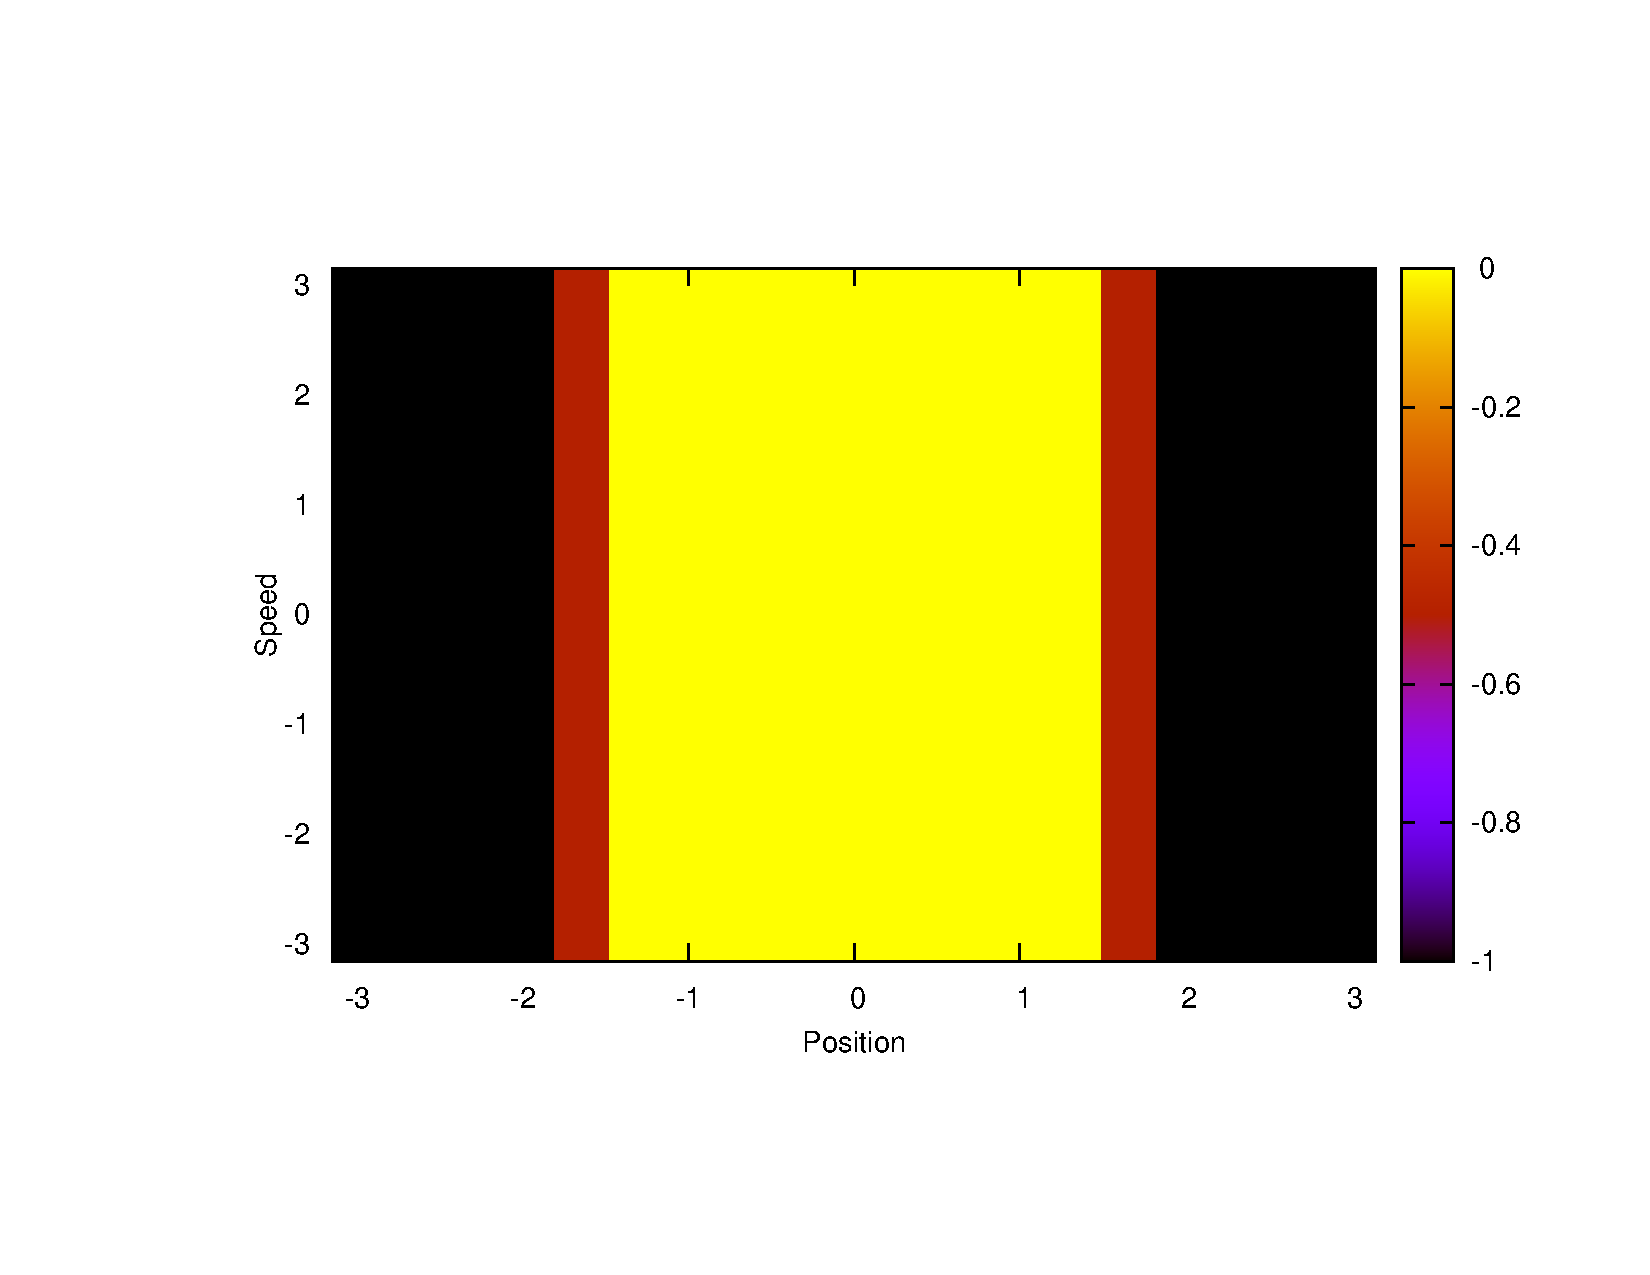
\includegraphics[width=\columnwidth]{LAFEM_Exp3_true_R.pdf}}
  \centerline{(a) Expert reward ($R^E$)}%\medskip
\end{minipage}
%\hfill
\begin{minipage}[b]{.48\linewidth}
  \centering
  \centerline{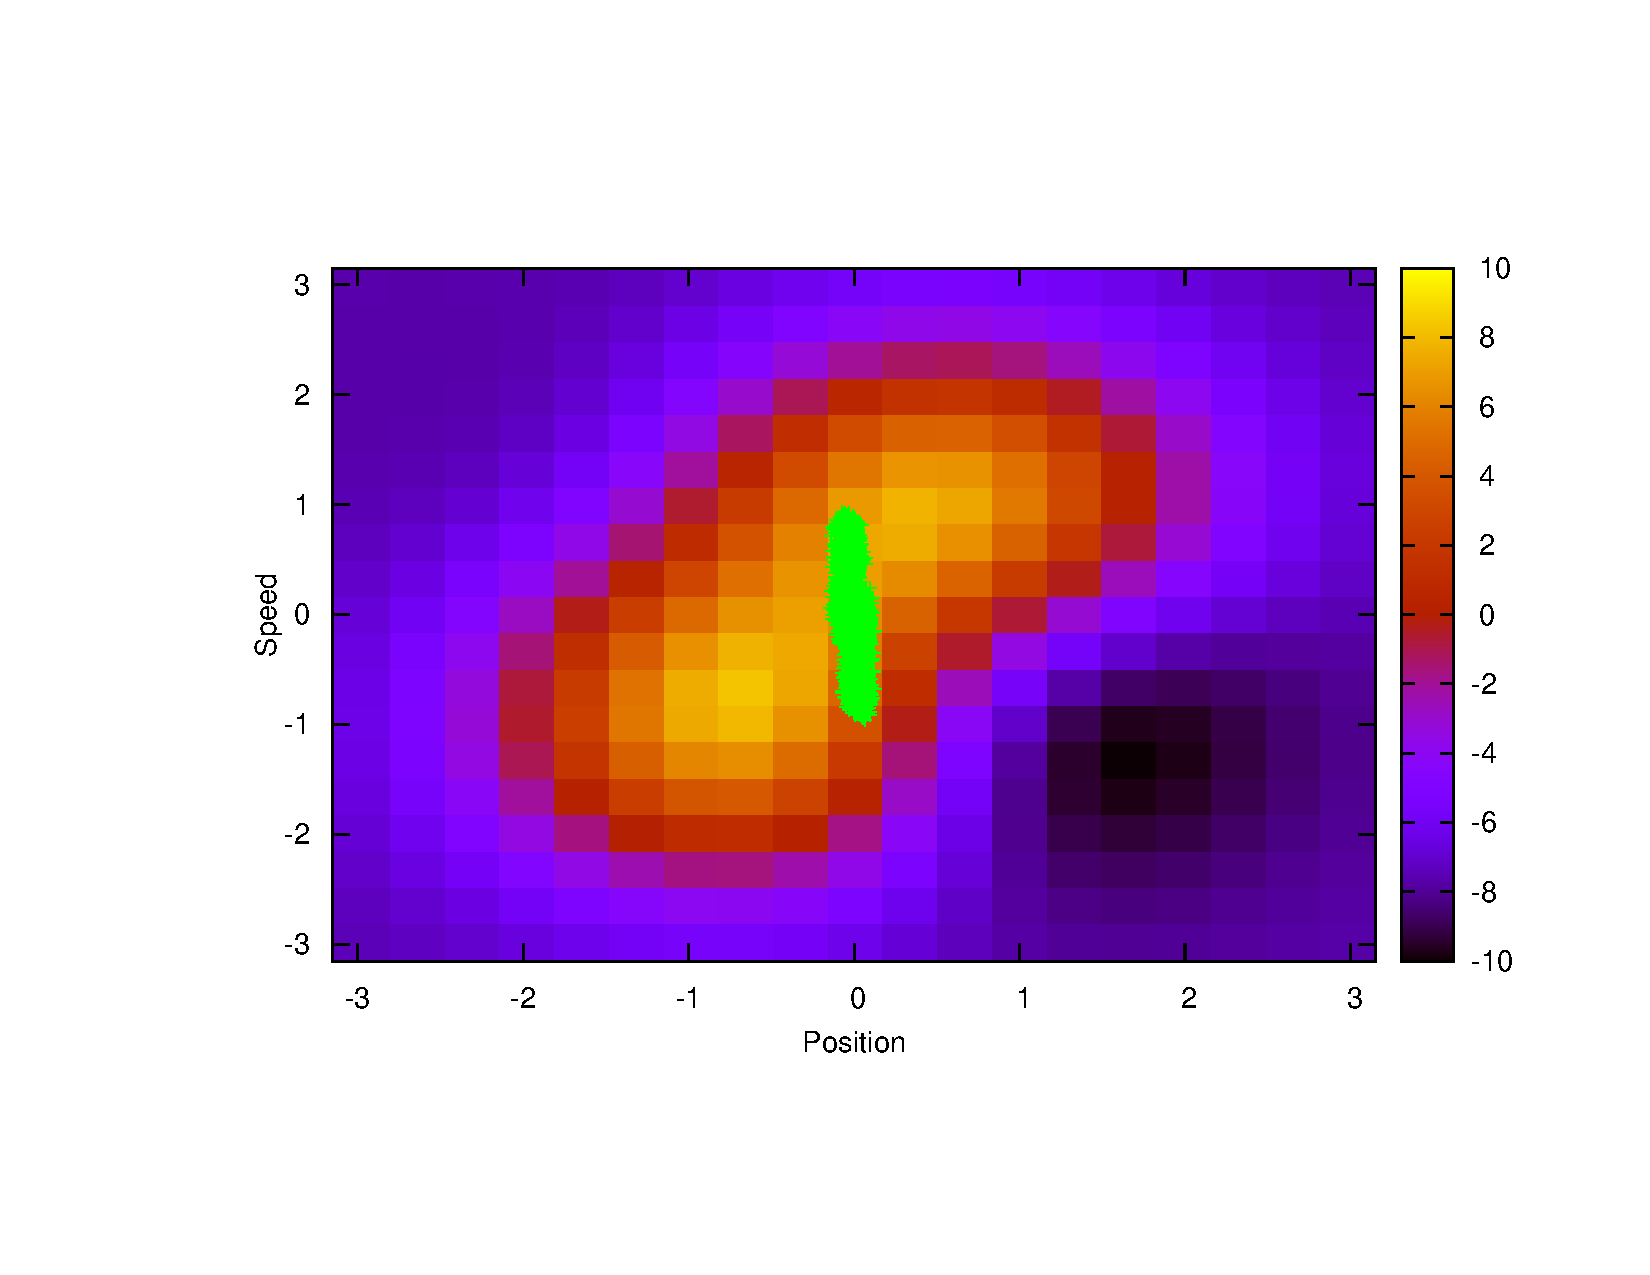
\includegraphics[width=\columnwidth]{LAFEM_Exp3_lafem_R.pdf}}
  \centerline{(b) SCIRL Reward ($R_\theta$)}%\medskip
\end{minipage}
\begin{minipage}[b]{.48\linewidth}
  \centering
  \centerline{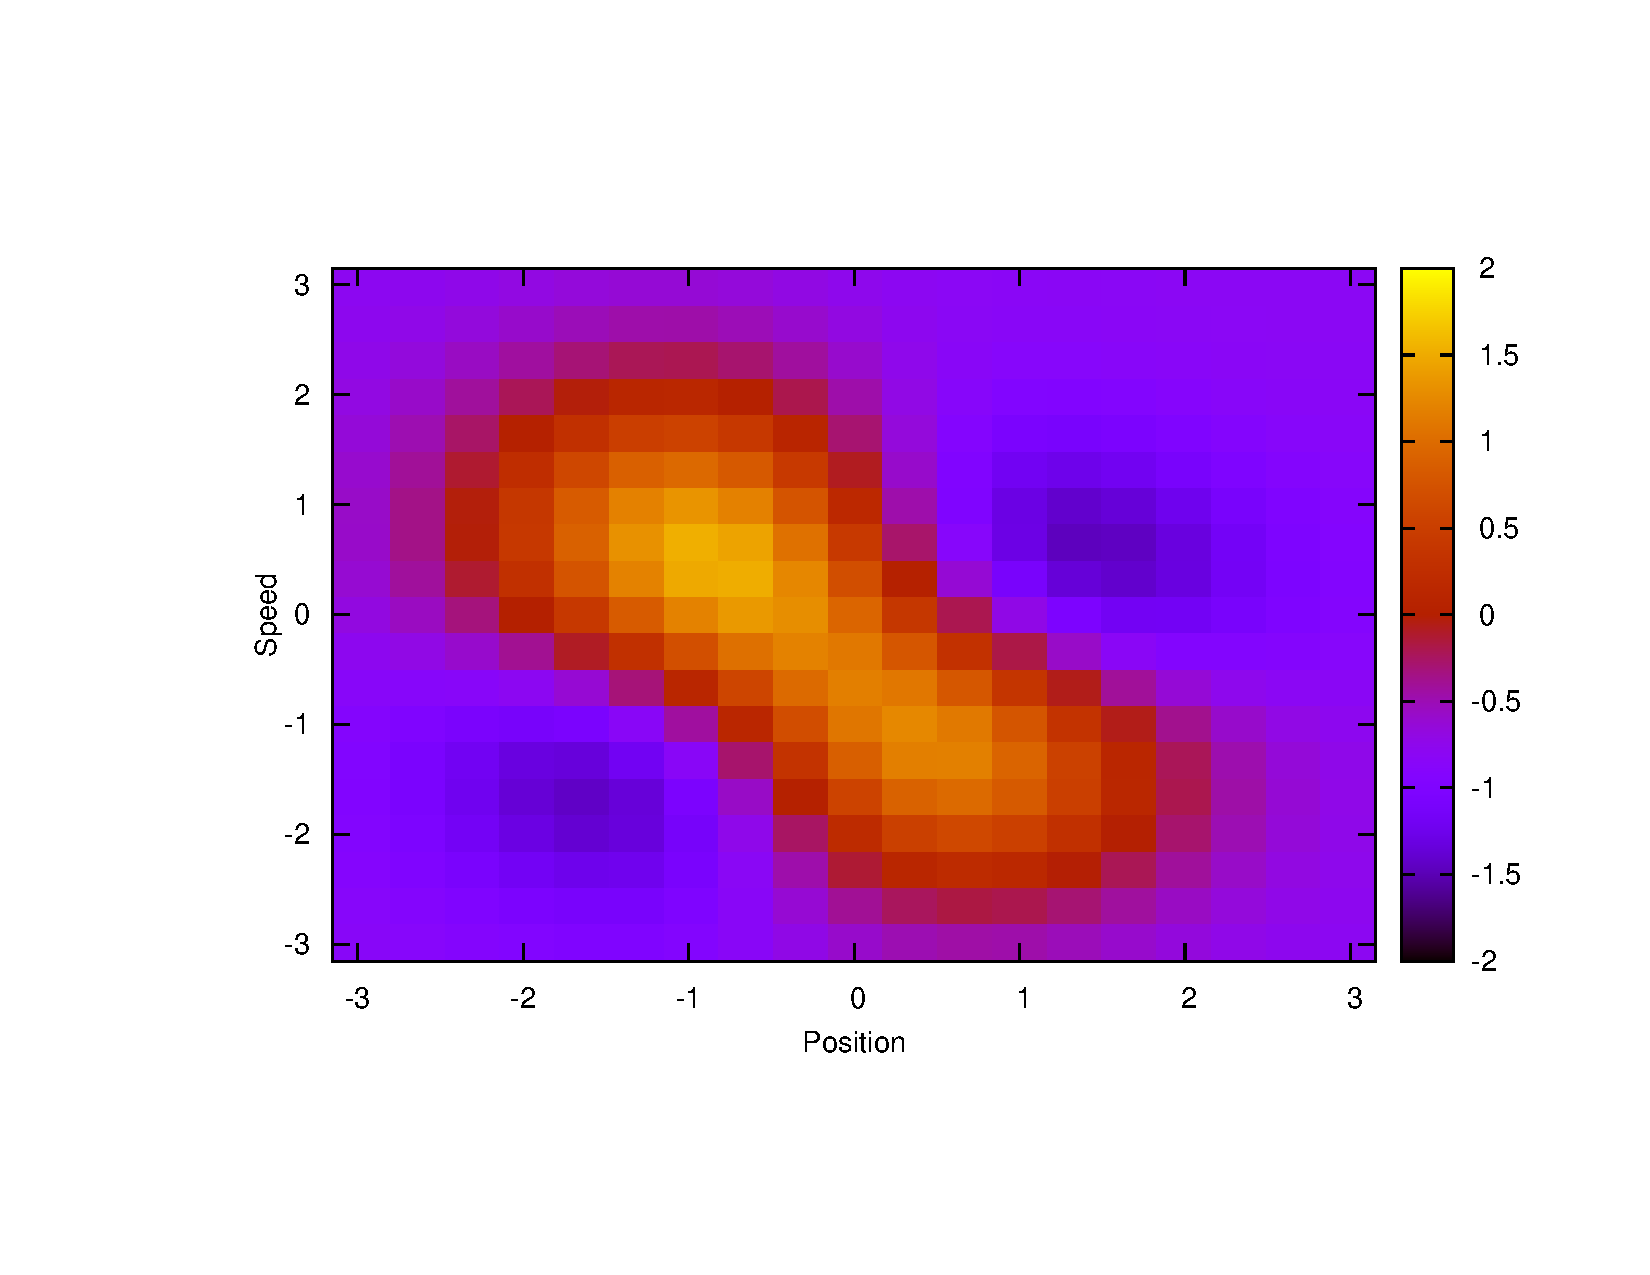
\includegraphics[width=\columnwidth]{LAFEM_Exp3_Vexpert.pdf}}
  \centerline{(c) Expert value function}%\medskip
\end{minipage}
\hfill
\begin{minipage}[b]{.48\linewidth}
  \centering
  \centerline{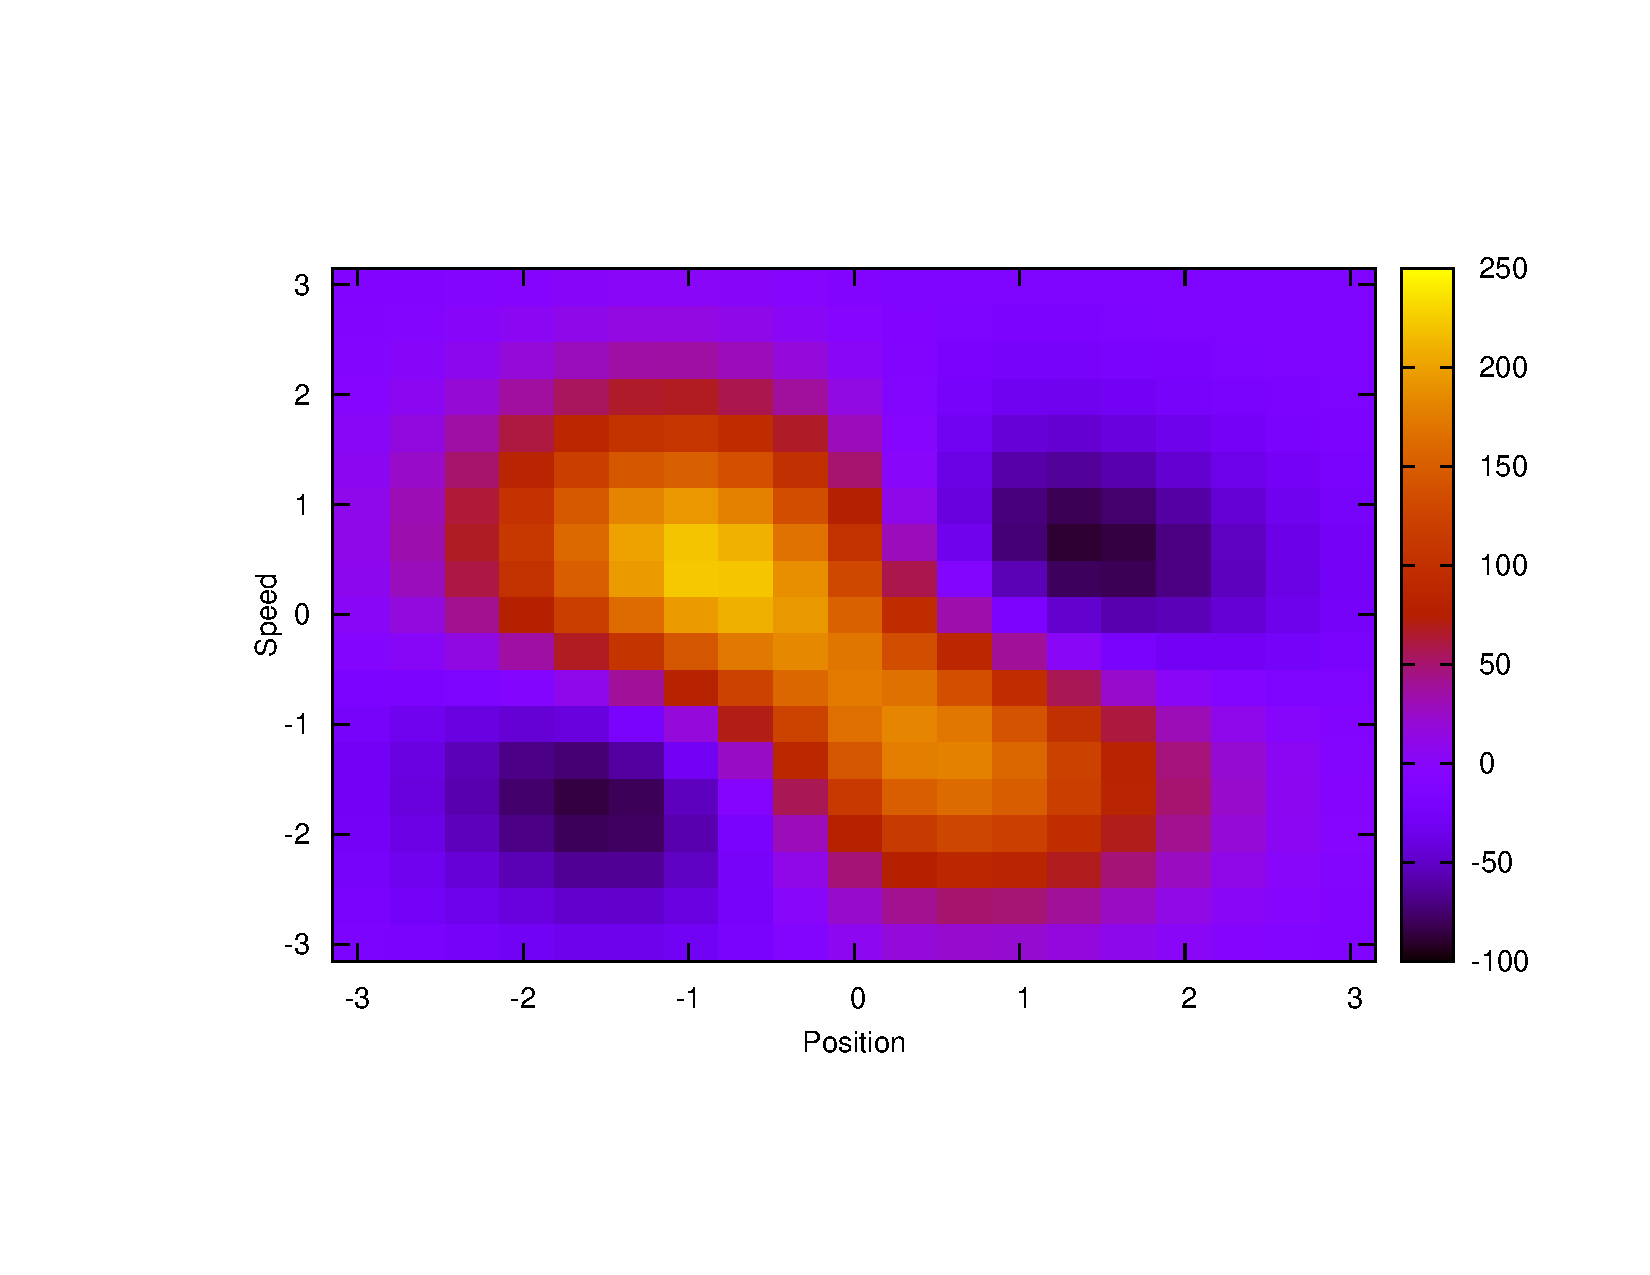
\includegraphics[width=\columnwidth]{LAFEM_Exp3_Vagent.pdf}}
  \centerline{(d) SCIRL value function}%\medskip
\end{minipage}
%
\caption{SCIRL results on the inverted pendulum} \label{onlyFig.fig}
%
\end{center}
\vskip -0.2in
\end{figure}
%
%Afin d'étudier le comportement de notre algorithme, nous avons fait générer à l'expert une base de données $D_E$ de transitions contenant 10 trajectoires de 300 transitions chacune.
%La fonction $l$ fut définie sur les états présents dans $D_E$ telle que $l(s,a) = 0$ si $a=\pi_E(s)$, $1$ sinon. Le pas de temps est constant à $\alpha_t = 0.1$ et le nombre d'itérations
%est de $T=20$. Le vecteur initial $\theta_0$ fut fixé à $[-1...-1]^T$, la récompense étant paramétrée à l'aide du vecteur d'attribut $\psi: S \rightarrow \mathbb{R}^p$ correspondant au mélange
%de gaussiennes défini dans \cite{lagoudakis2003least}. Pour l'approximation de l'attribut vectoriel moyen de l'expert, c'est l'algorithme LSTD$\mu$ qui fut employé.\\
%
So as to test the SCIRL algorithm, a database $D_E$ of transitions
given by the expert policy $\pi_E$ is built. It contains 10
trajectories of 300 transitions each. The margin function is $l(s,a)
= 0$ if $a=\pi_E(s)$, $1$ otherwise.
%The time step is constant,
%$\Delta t=0.1s$, and the stopping time is $T=20$.
The initial vector, $\theta_0$, is fixed at $\begin{pmatrix}   -1 &
\dots & -1
\end{pmatrix}^T$,
and the basis functions ($\psi: S \rightarrow \mathbb{R}^p$) used
for the reward function are a Gaussian network as defined
in~\cite{lagoudakis2003least}. The LSTD$\mu$
algorithm~\cite{klein2011batch} is used to estimate the feature
expectation $\mu^E(s,a)$.

%Si la fonction de récompense trouvée par LAFEM (figure \ref{onlyFig.fig} (b)) diffère de celle fournie à l'expert (figure \ref{onlyFig.fig} (a)) on constate en revanche que les fonctions de valeurs
%sont très similaires (figures \ref{onlyFig.fig} (c) et \ref{onlyFig.fig} (d)). Cela est une illustration du fait que le problème de l'ARI est mal posé en ceci qu'il n'y a pas qu'une seule récompense
%pouvant expliquer une politique.\\
%
Even if the reward function found by SCIRL (figure \ref{onlyFig.fig}
(b)) is different than the expert reward (figure \ref{onlyFig.fig}
(a)), the value functions are similar (figures \ref{onlyFig.fig} (c)
et \ref{onlyFig.fig} (d)). This is an illustration that the IRL
problem is ill-posed in the sense that there is not only one reward
function able to explain the optimality of a policy.

%Avec le nombre d'échantillons fournis par l'expert (3000 en 10 trajectoires de 300 transitions chacune), l'agent parvient systématiquement à maintenir le pendule en équilibre durant 5 minutes,
%ce qui est notre critère de réussite.\\
With the number of samples given by the expert (3000), the
apprentice is able to systematically maintain the pendulum in
equilibrium during 5 minutes as the expert does.
%
%Deux éléments méritent d'être notés. Tout d'abord la faible couverture de l'espace d'état offerte par les échantillons de l'expert.
%Ceux-ci sont portés en vert sur la Figure \ref{onlyFig.fig} (b) et l'on constate qu'ils n'occupent qu'une toute petite partie de l'espace:
%celle dans laquelle le pendule est proche de la verticale. En l'absence de données dans le reste de l'espace d'état il n'est pas possible de pouvoir y inférer avec certitude la récompense.
%Le second point à noter est que la "vraie" récompense ne se trouve pas dans l'espace d'hypothèse que notre algorithme explore, en effet les attributs vectoriels utilisés ne peuvent qu'approximer
%la fonction de récompense utilisée sans l'atteindre. Malgré ces deux difficultés, notre algorithme parvient, comme nous l'avons dit, à extraire une récompense qui permet à un agent d'obtenir
%des performances similaires à celles de l'expert. Le lecteur attentif aura noté la différence d'amplitude des fonctions de valeur Fig. \ref{onlyFig.fig} Cela n'a aucune importance, une dilatation
%laissant la politique optimale invariante.
%
Two elements deserve to be noticed. First, the expert samples are
only covering a small area of the state space (see
Figure~\ref{onlyFig.fig} (b)) and especially they are close to the
vertical position. The lack of samples in the rest of the state
space makes it impossible to infer with certainty the reward
function. Second, the \textit{actual} reward function $R^E$
(Figure~\ref{onlyFig.fig} (a)) doesn't live in the hypothesis space
span by a linear combination of the basis functions. Despite these
difficulties, SCIRL succeeds to extract a reward function leading to
perform similarly to the expert. %Notice that there is a magnitude
%difference between the SCIRL and the expert value functions on
%Figure~\ref{onlyFig.fig} but an affine transform of the value
%function does not change the optimal policies.

\subsection{Car driving}

This task is taken from~\cite{syed2008game}. It consists in
navigating a car through randomly-generated traffic on a threelane
highway. The reward features are identical to~\citet{syed2008game}
paper that is: a collision feature (0 if contact with another car,
and 0.5 otherwise), an off-road feature (0 if on the grass, and 0.5
otherwise), and a speed feature (0.5, 0.75 and 1 for each of the
three possible speeds, with higher values corresponding to higher
speeds).

\subsubsection{Results}

In this section, SCIRL is compared to the Multiplicative Weights for
Apprenticeship Learning (MWAL) algorithm proposed by
\citet{syed2008game}. This algorithm requires the perfect knowledge
of the MDP and outputs a single policy (not a reward) that imitates
the expert.

The experimental setup is as follows. The highway simulator
of~\cite{syed2008game} is used\footnote{available at \url{
http://www.cs.princeton.edu/~usyed/}}. It also contains an exact MDP
solver for the task, the transition probabilities being available.
Two reward functions were hand-tuned ($\theta$ parameters chosen by
hand) so as to generate two different expert policies: one for
high-speed driving and another for safe driving. The MDP solver is
used to obtain the expert policies given the two reward functions. A
number $N$ of trajectories of length $H$ is generated with each
strategy providing the expert data for training the SCIRL and MWAL
algorithms. The MWAL algorithm requires the knowledge of the average
feature expectation $\mu_{d0}^{\pi_E}$ for the initial state (given
a distribution $d_0$ over starting states). To reach a fair
comparison with SCIRL which only uses the expert trajectories,
$\mu_{d_0}^{\pi_E}$ is computed as the Monte Carlo estimate given
the $N$ trajectories, knowing that the initial state is always the
same:
%
$$\mu_{d_0}^{\pi_E} = \frac{1}{N}\sum_{i=1}^N \sum_{t=1}^H \gamma^t \psi(s_t^i)$$
%
For SCIRL, the LSTD$\mu$ algorithm is used again to approximate
$\mu^E(s,a)$ from the data. For each component of $\mu^E$, the basis
functions are the same as those for the reward function. SCIRL
outputs a reward function which is used to obtain a policy using the
MDP solver. The SCIRL and MWAL policies are then run on the
simulator for trajectories of length $T$. The average discounted
cumulative reward, computed with regard to the initial handcrafted
rewards, serves as the performance measure. It is an Monte Carlo
estimate of $V^\pi(s_0)$ for each policy.

This experiment is repeated $M$ times for each policy and results
are averaged. The results are shown in
Tables~\ref{table:highway_fast} and~\ref{table:highway_safe}
 for $N \in
\{1, 3, 5, 10\}$, $H = 30$, $T=50$ and $M = 10$.

%\begin{figure}
%  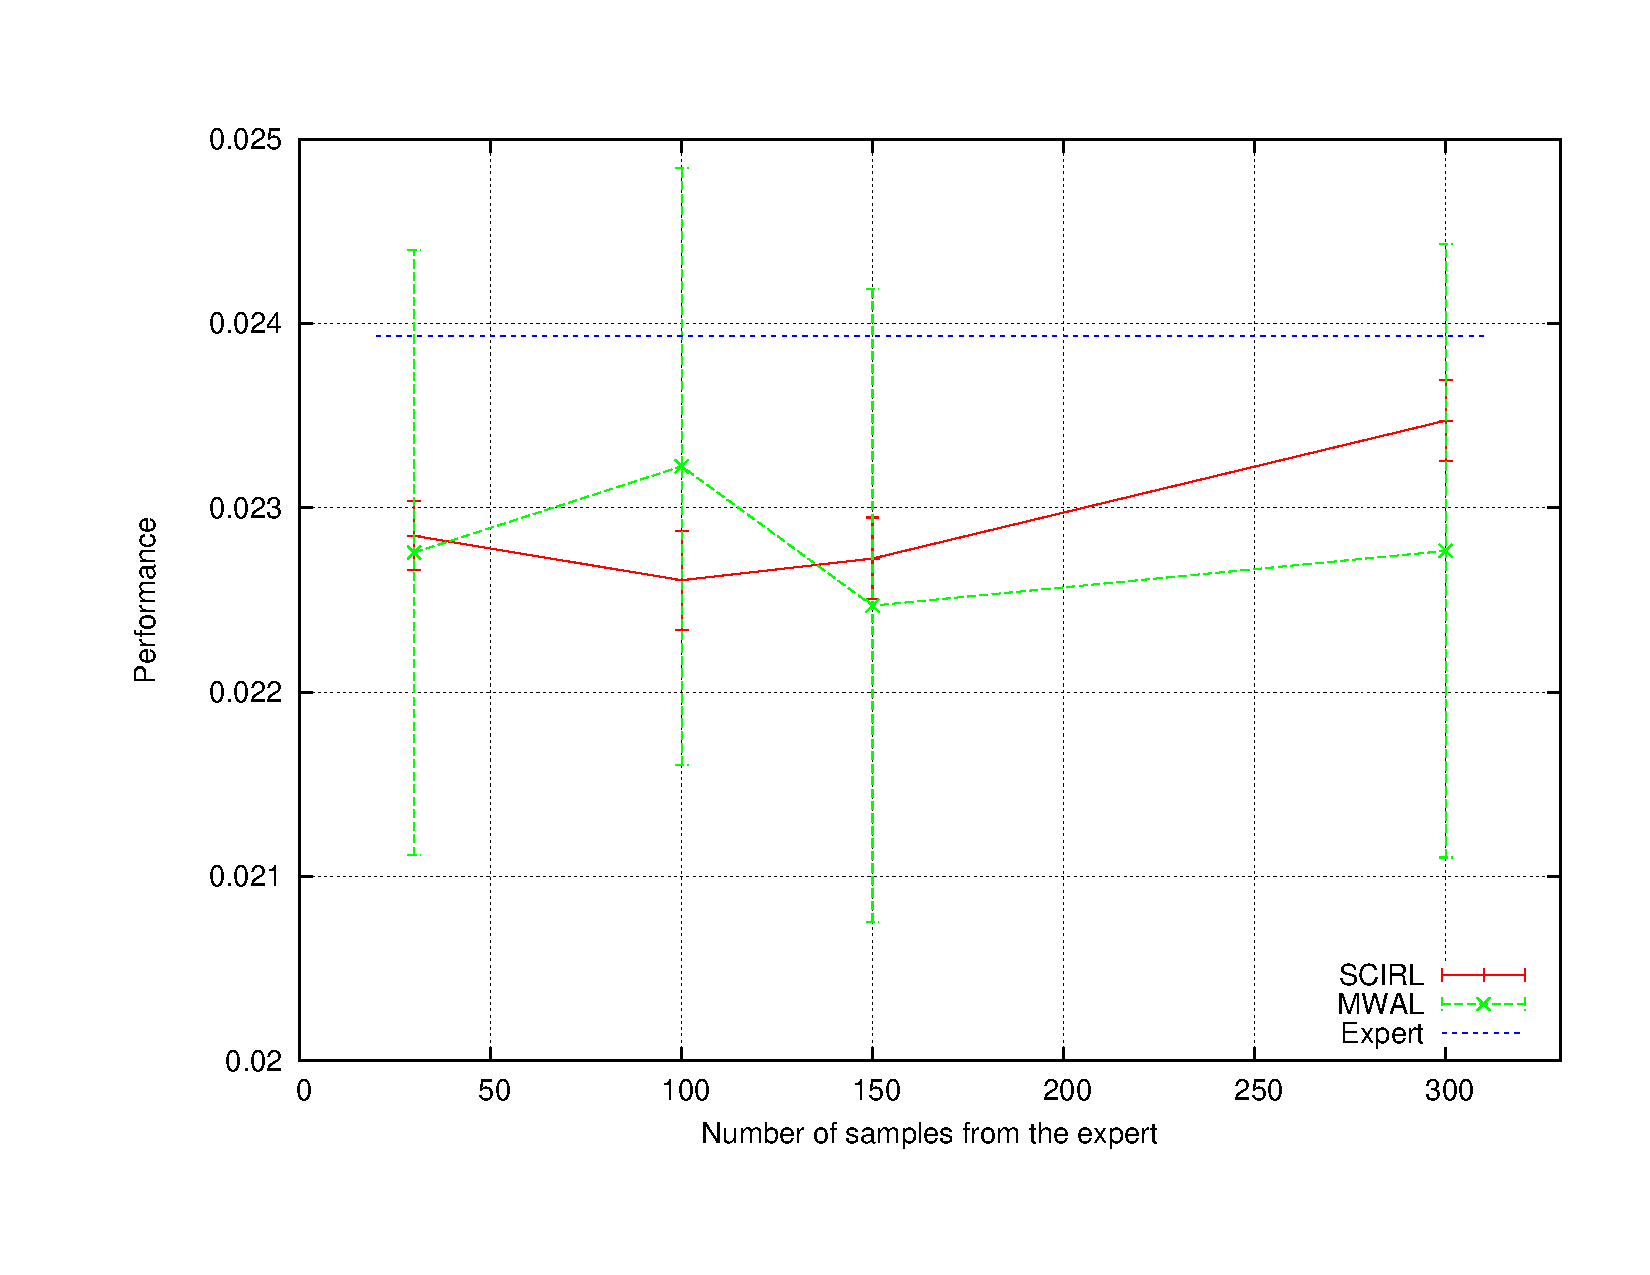
\includegraphics[width=\linewidth]{FastResults_EB.pdf}\\
%  \caption{Results for high-speed driving}\label{fig:highway_fast}
%\end{figure}
%
%\begin{figure}
%  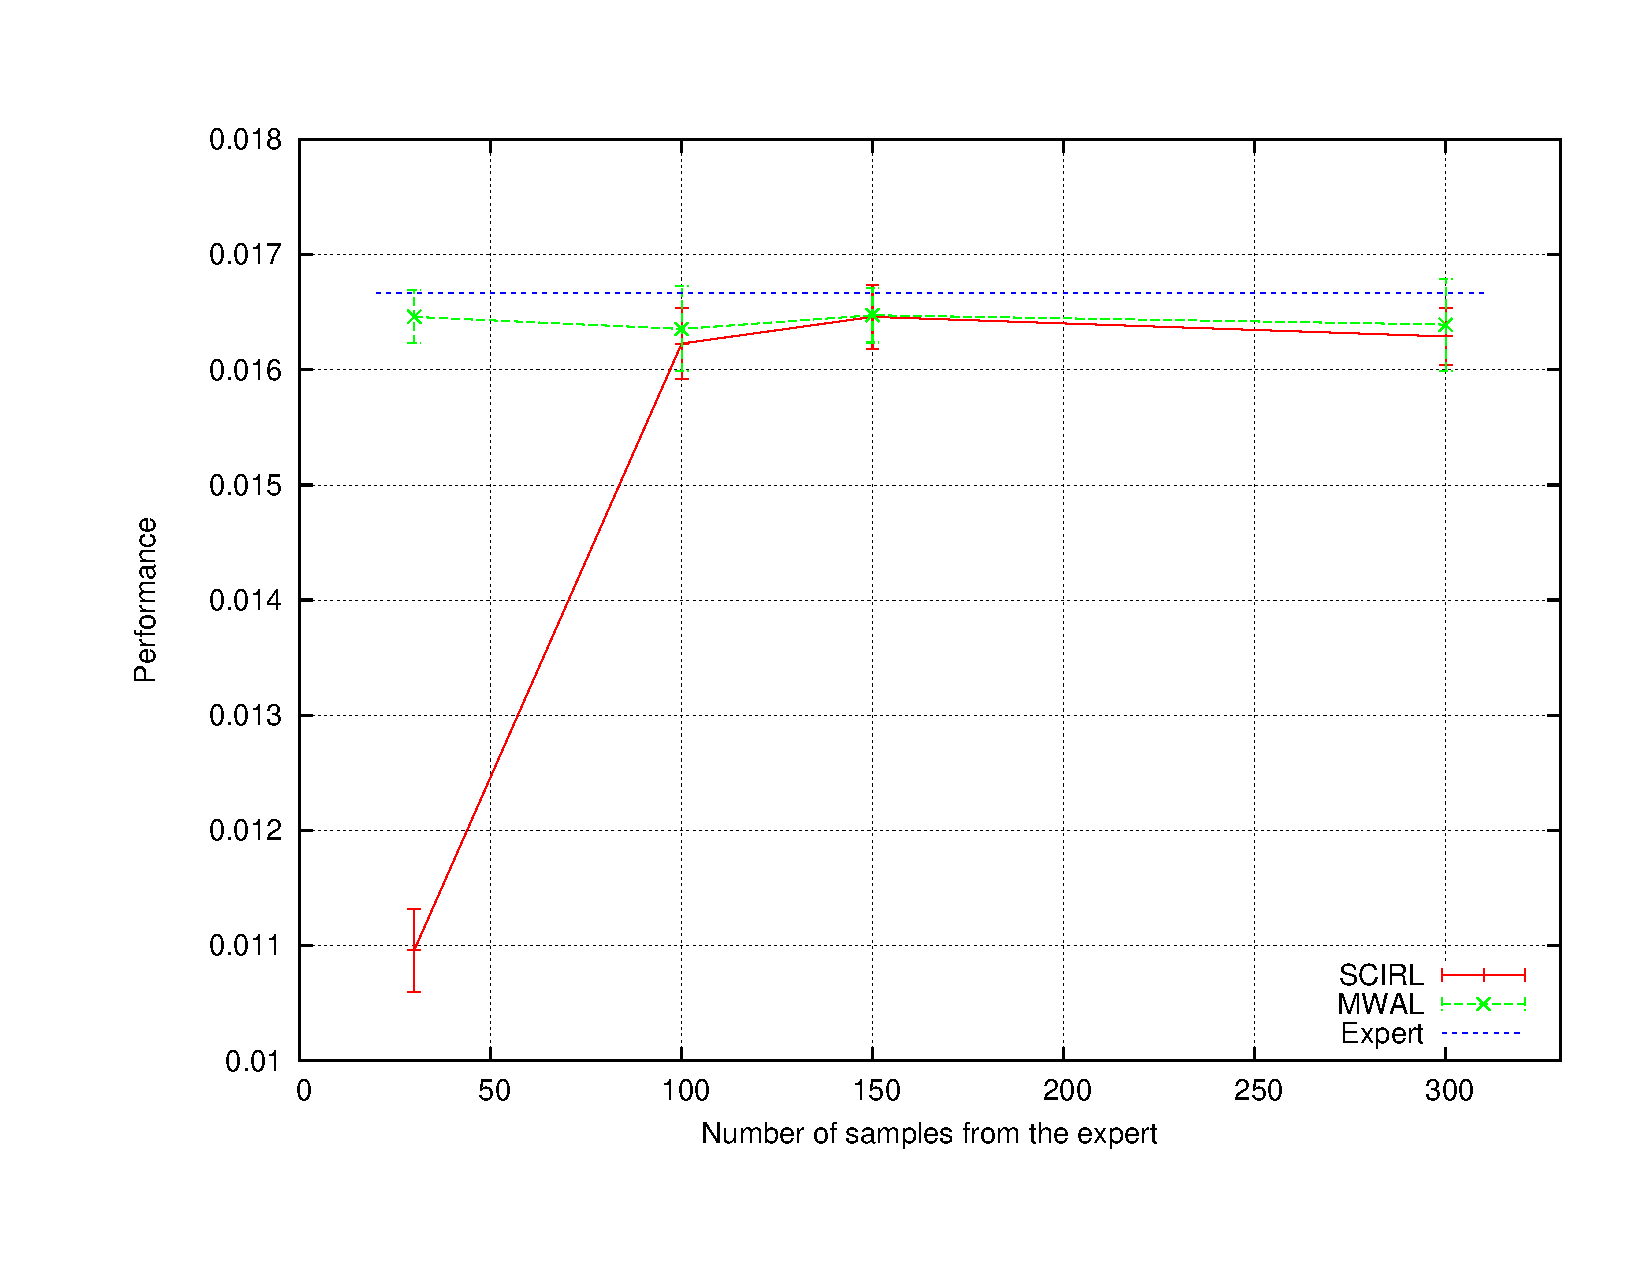
\includegraphics[width=\linewidth]{SafeResults_EB.pdf}\\
%  \caption{Results for high-speed driving}\label{fig:highway_safe}
%\end{figure}

\begin{table}
\begin{center}
    \begin{tabular}{|c|c|c|c|}
    \hline
    % after \\: \hline or \cline{col1-col2} \cline{col3-col4} ...
    N     & MWAL              & SCIRL               & $V_{\text{opt}}$ \\\hline\hline
    1     & 7.25 $\pm$ 0.10   & 7.03 $\pm$ 0.09     & 7.30              \\\hline
    3     & 7.28 $\pm$ 0.06   & 7.07 $\pm$ 0.07     & 7.30              \\\hline
    5     & 7.27 $\pm$ 0.11   & 6.98 $\pm$ 0.10     & 7.30              \\\hline
    10    & 7.26 $\pm$ 0.07   & 7.05 $\pm$ 0.10     & 7.30              \\
    \hline
    \end{tabular}
    \caption{SCIRL results on the car driving
    problem (high-speed)}\label{table:highway_fast}
\end{center}
\end{table}

\begin{table}
\begin{center}
    \begin{tabular}{|c|c|c|c|}
    \hline
    % after \\: \hline or \cline{col1-col2} \cline{col3-col4} ...
    N     & MWAL              & SCIRL               & $V_{\text{opt}}$ \\\hline\hline
    1     & 4.95 $\pm$ 0.05   & 3.27 $\pm$ 0.13     & 5.00              \\\hline
    3     & 4.85 $\pm$ 0.13   & 4.90 $\pm$ 0.10     & 5.00              \\\hline
    5     & 4.90 $\pm$ 0.09   & 4.83 $\pm$ 0.08     & 5.00              \\\hline
    10    & 4.98 $\pm$ 0.03   & 4.81 $\pm$ 0.12     & 5.00              \\
    \hline
    \end{tabular}
    \caption{SCIRL results on the car driving
    problem (safe)}\label{table:highway_safe}
\end{center}
\end{table}


From these tables, one can conclude that the SCIRL method reaches
approximately the same performance as MWAL (given that enough
samples are provided in the case of safe driving). Yet, SCIRL
doesn't need any other information than the expert demonstrations
while MWAL requires solving exactly and repeatedly the MDP.

\section{Conclusion}

%L'algorithme présenté dans cette contribution lève les problèmes les plus contraignants de l'apprentissage par renforcement inverse. En rendant la résolution du problème inverse indépendante
%de celle du problème direct, nous sommes en mesure d'inférer une récompense cohérente avec le comportement d'un expert en mode purement \emph{batch}.\\
In this paper, we propose an algorithm for inverse reinforcement
learning (IRL) that we call SCIRL. It is based on a classification
approach in which the structure of the underlying Markov Decision
Process (MDP) is taken into account.

This approach relaxes most of the constrains of other IRL algorithms
found in the literature. It doesn't require the resolution of the
direct problem and is able to infer a reward function which is
consistent with the expert's behavior in a purely \emph{batch} mode.
%
%Comme nous l'avons illustré, les échantillons nécessaires à la réussite de notre algorithmes sont faciles à recueillir.
%Une simple trace de l'expert, même si elle ne couvre qu'une petite partie de l'espace d'état, suffit à inférer une récompense.
%Cette récompense, description compacte de la tâche effectuée par l'expert, peut alors être optimisée par un agent dont les capacités diffèrent de celles de l'expert.
%On rentre dans le cadre du \emph{transfer learning}.\\
%
A mere trajectory of the expert, even if it covers a small part of
the state space, is sufficient to infer a reward function and no
additional data nor a simulator is required. It also outputs a
reward and not a strategy which is the real goal of the IRL
paradigm. The learnt reward function, which is a compact description
of the task executed by the expert, could then be optimized by an
agent with abilities (action set) that are different from those of
the expert which places us in in the even more challenging framework
of \emph{transfer learning}.
%
%L'estimation de $\mu_E$ est centrale dans notre approche. Nous disposons d'un algorithme efficace avec LSTD$\mu$, mais qui présente cependant les mêmes inconvénients
%que les algorithmes d'estimation d'une fonction de valeur. L'axe d'étude que nous envisageons d'explorer serait de ne plus passer par l'attribut vectoriel moyen en trouvant le moyen
%d'introduire autrment la structure du PDM dans la démarche de classification que nous avons adoptée. Des tests empiriques sur des problèmes plus comlpexes sont également envisagés.

SCIRL is shown to compare positively to a state-of-the-art algorithm
(the MWAL algorithm) on a standard benchmark (the car driving
problem). It also performs well on a problem with a two-dimensional
continuous state space which is sparsely explored by the expert (the
inverted pendulum problem). This later problem could not be solved
with state-of-the-art algorithms without additional knowledge.

Yet, SCIRL requires the computation of $\mu^E(s,a)$ everywhere on
the expert trajectories. Here, we made use of the LSTD$\mu$
algorithm to estimate it. However LSTD$\mu$ shares the drawbacks of
value function estimation algorithms. In the future, we plan to
extend our approach so as to avoid the computation of the expert's
feature expectations. Empirical tests on more complex problems will
also be considered.

\bibliography{Biblio}
\bibliographystyle{icml2012}
\end{document}
